\documentclass{article}

% All packages, macros and the abbreviation database live in separate files.
\usepackage{fontspec}
\usepackage[vietnamese,main=english]{babel}
\usepackage[a4paper,top=2.5cm,bottom=2.5cm,left=3cm,right=2cm]{geometry}
\usepackage{amsmath}
\usepackage{booktabs,array,tabularx,xltabular}
\usepackage{graphicx}
\usepackage{enumitem}
\usepackage{longtable}
\usepackage{tikz}
\usetikzlibrary{arrows.meta,positioning,calc}
\usepackage[
  colorlinks=true,
  linkcolor=blue,
  citecolor=blue,
  urlcolor=blue
]{hyperref}
\usepackage{acro}[=v3]
\acsetup{make-links=true}

% Thu muc chua anh minh chung (sao chep tu My Drive > Networking > picture source).
\graphicspath{{figures/}}

% =====================================================================
% acronyms.tex -- abbreviation database for the acro package
% Use \ac{key} (first use expands), \acp{key} (plural), \acs{key} (short).
% =====================================================================

% --- Networks and organisations ---
\DeclareAcronym{wlan}{short = WLAN, long = {Wireless Local Area Network}}
\DeclareAcronym{lan}{short = LAN, long = {Local Area Network}}
\DeclareAcronym{wpan}{short = WPAN, long = {Wireless Personal Area Network}}
\DeclareAcronym{wwan}{short = WWAN, long = {Wireless Wide Area Network}}
\DeclareAcronym{ieee}{short = IEEE, long =
  {Institute of Electrical and Electronics Engineers}}
\DeclareAcronym{iot}{short = IoT, long = {Internet of Things}}

% --- Architecture ---
\DeclareAcronym{ap}{short = AP, long = {Access Point}}
\DeclareAcronym{sta}{short = STA, long = {Station}}
\DeclareAcronym{bss}{short = BSS, long = {Basic Service Set}}
\DeclareAcronym{bssid}{short = BSSID, long = {Basic Service Set Identifier}}
\DeclareAcronym{ibss}{short = IBSS, long = {Independent Basic Service Set}}
\DeclareAcronym{ess}{short = ESS, long = {Extended Service Set}}
\DeclareAcronym{ssid}{short = SSID, long = {Service Set Identifier}}
\DeclareAcronym{ds}{short = DS, long = {Distribution System}}
\DeclareAcronym{wlc}{short = WLC, long = {Wireless LAN Controller}}
\DeclareAcronym{capwap}{short = CAPWAP, long =
  {Control And Provisioning of Wireless Access Points}}
\DeclareAcronym{poe}{short = PoE, long = {Power over Ethernet}}
\DeclareAcronym{vlan}{short = VLAN, long = {Virtual Local Area Network}}

% --- Radio and PHY ---
\DeclareAcronym{ism}{short = ISM, long = {Industrial, Scientific and Medical}}
\DeclareAcronym{phy}{short = PHY, long = {Physical (layer)}}
\DeclareAcronym{dsss}{short = DSSS, long = {Direct-Sequence Spread Spectrum}}
\DeclareAcronym{fhss}{short = FHSS, long = {Frequency-Hopping Spread Spectrum}}
\DeclareAcronym{cck}{short = CCK, long = {Complementary Code Keying}}
\DeclareAcronym{ofdm}{short = OFDM, long =
  {Orthogonal Frequency-Division Multiplexing}}
\DeclareAcronym{ofdma}{short = OFDMA, long =
  {Orthogonal Frequency-Division Multiple Access}}
\DeclareAcronym{mimo}{short = MIMO, long = {Multiple-Input Multiple-Output}}
\DeclareAcronym{mumimo}{short = MU-MIMO, long = {Multi-User MIMO}}
\DeclareAcronym{dfs}{short = DFS, long = {Dynamic Frequency Selection}}
\DeclareAcronym{tpc}{short = TPC, long = {Transmit Power Control}}
\DeclareAcronym{ru}{short = RU, long = {Resource Unit}}
\DeclareAcronym{mlo}{short = MLO, long = {Multi-Link Operation}}
\DeclareAcronym{twt}{short = TWT, long = {Target Wake Time}}
\DeclareAcronym{eirp}{short = EIRP, long =
  {Equivalent Isotropically Radiated Power}}
\DeclareAcronym{psd}{short = PSD, long = {Power Spectral Density}}

% --- MAC ---
\DeclareAcronym{mac}{short = MAC, long = {Medium Access Control}}
\DeclareAcronym{csmaca}{short = CSMA/CA, long =
  {Carrier-Sense Multiple Access with Collision Avoidance}}
\DeclareAcronym{ampdu}{short = A-MPDU, long = {Aggregate MPDU}}
\DeclareAcronym{edca}{short = EDCA, long =
  {Enhanced Distributed Channel Access}}
\DeclareAcronym{qos}{short = QoS, long = {Quality of Service}}
\DeclareAcronym{wmm}{short = WMM, long = {Wi-Fi Multimedia}}
\DeclareAcronym{rrm}{short = RRM, long = {Radio Resource Management}}
\DeclareAcronym{btm}{short = BTM, long = {BSS Transition Management}}
\DeclareAcronym{fils}{short = FILS, long = {Fast Initial Link Setup}}

% --- Security ---
\DeclareAcronym{wep}{short = WEP, long = {Wired Equivalent Privacy}}
\DeclareAcronym{wpa}{short = WPA, long = {Wi-Fi Protected Access}}
\DeclareAcronym{tkip}{short = TKIP, long = {Temporal Key Integrity Protocol}}
\DeclareAcronym{ccmp}{short = CCMP, long = {Counter Mode with CBC-MAC Protocol}}
\DeclareAcronym{gcmp}{short = GCMP, long = {Galois/Counter Mode Protocol}}
\DeclareAcronym{aes}{short = AES, long = {Advanced Encryption Standard}}
\DeclareAcronym{psk}{short = PSK, long = {Pre-Shared Key}}
\DeclareAcronym{sae}{short = SAE, long =
  {Simultaneous Authentication of Equals}}
\DeclareAcronym{owe}{short = OWE, long = {Opportunistic Wireless Encryption}}
\DeclareAcronym{pmf}{short = PMF, long = {Protected Management Frames}}
\DeclareAcronym{pmk}{short = PMK, long = {Pairwise Master Key}}
\DeclareAcronym{ptk}{short = PTK, long = {Pairwise Transient Key}}
\DeclareAcronym{gtk}{short = GTK, long = {Group Temporal Key}}
\DeclareAcronym{mic}{short = MIC, long = {Message Integrity Code}}
\DeclareAcronym{eap}{short = EAP, long = {Extensible Authentication Protocol}}
\DeclareAcronym{eapol}{short = EAPOL, long = {EAP over LAN}}
\DeclareAcronym{radius}{short = RADIUS, long =
  {Remote Authentication Dial-In User Service}}
\DeclareAcronym{tls}{short = TLS, long = {Transport Layer Security}}
\DeclareAcronym{peap}{short = PEAP, long = {Protected EAP}}
\DeclareAcronym{dpp}{short = DPP, long = {Device Provisioning Protocol}}
\DeclareAcronym{wips}{short = WIPS, long =
  {Wireless Intrusion Prevention System}}
\DeclareAcronym{krack}{short = KRACK, long = {Key Reinstallation Attack}}
\DeclareAcronym{wps}{short = WPS, long = {Wi-Fi Protected Setup}}

% --- Regulatory & Miscellaneous (Vietnam) ---
\DeclareAcronym{vnmic}{short = MIC, long =
  {Ministry of Information and Communications}}
\DeclareAcronym{qcvn}{short = QCVN, long =
  {Quy chuẩn kỹ thuật quốc gia (National Technical Regulation)}}
\DeclareAcronym{uas}{short = UAS, long = {Unmanned Aircraft Systems}}
\DeclareAcronym{doc}{short = DoC, long = {Declaration of Conformity}}


% Tóm tắt ngắn.
\newenvironment{tomtat}{%
  \par\medskip\noindent
  \begin{minipage}{\linewidth}%
    \hrule\smallskip
    \noindent\textbf{Tóm tắt}\par\nopagebreak
    \begin{itemize}[nosep,leftmargin=*]%
      }{%
    \end{itemize}%
    \smallskip\hrule
  \end{minipage}\par\medskip
}


\begin{document}
\begin{titlepage}
  \centering
  {\large ĐẠI HỌC QUỐC GIA THÀNH PHỐ HỒ CHÍ MINH\par}
  \vspace{0.2cm}
  {\large TRƯỜNG ĐẠI HỌC KHOA HỌC TỰ NHIÊN\par}
  \vspace{0.2cm}
  {\large KHOA CÔNG NGHỆ THÔNG TIN\par}
  \vspace{1.6cm}
  {\large CTT105 -- MẠNG MÁY TÍNH\par}
  \vspace{0.5cm}
  {\Large\bfseries ĐỒ ÁN WLAN\par}
  \vspace{0.25cm}
  {\huge\bfseries MẠNG CỤC BỘ KHÔNG DÂY\par}
  {\Large (Wireless Local Area Network -- WLAN)\par}
  \vspace{0.6cm}
  {\Large Nhóm 9 -- Mạng máy tính\par}
  \vspace{0.5cm}
  {\large\bfseries Thông tin thành viên\par}
  \vspace{0.2cm}
  \renewcommand{\arraystretch}{1.6}
  \begin{tabularx}{\linewidth}{c X X}
    \toprule
    STT & MSSV & Họ và tên \\
    \midrule
    1 & & \\
    2 & & \\
    3 & & \\
    4 & & \\
    5 & & \\
    6 & & \\
    \bottomrule
  \end{tabularx}
  \vfill
  {\large Giảng viên hướng dẫn: \rule{6.5cm}{0.4pt}\par}
  \vspace{0.4cm}
  {\large Thành phố Hồ Chí Minh, 2026\par}
\end{titlepage}


\begin{abstract}
  Báo cáo trình bày cơ sở lý thuyết về mạng cục bộ không dây (Wireless Local
  Area Network -- WLAN), gồm các thế hệ Wi-Fi, tiêu chuẩn IEEE 802.11, phổ tần
  và quy hoạch kênh, kiến trúc triển khai, cùng các cơ chế và vấn đề bảo mật.
  Phần thực nghiệm được dành chỗ để nhóm bổ sung sau. Phụ lục cung cấp danh
  sách từ viết tắt và bảng thuật ngữ chuyên ngành Anh--Việt.
\end{abstract}

\tableofcontents
\clearpage
\listoffigures
\listoftables
\clearpage

% ---------------- Main matter (one file per part) ----------------
% =====================================================================
% 01_introduction.tex
% =====================================================================
\begingroup
\newcolumntype{L}[1]{>{\hsize=#1\hsize\raggedright\arraybackslash}X}

\section{Tổng quan về mạng cục bộ không dây}
\label{sec:intro}

\subsection{WLAN là gì?}

\ac{wlan} là mạng dữ liệu kết nối các thiết bị thông qua môi trường vô tuyến
thay vì cáp, thường được triển khai trong nhà ở, văn phòng, khuôn viên trường
học hoặc địa điểm công cộng. Hầu hết \acp{wlan} hiện nay đều dựa trên họ tiêu
chuẩn \ac{ieee} 802.11, quy định các lớp \ac{phy} và \ac{mac}
  \cite{ieee80211_2020,kurose2012,hcmus_wlan_report}.

\subsection{LAN và WLAN}

\ac{lan} kết nối các thiết bị trong một phạm vi giới hạn, thường sử dụng
Ethernet chuyển mạch và cáp vật lý. \ac{wlan} cung cấp chức năng mạng cục bộ
tương tự thông qua môi trường vô tuyến dùng chung, giúp người dùng di chuyển
linh hoạt và triển khai mạng dễ dàng hơn, nhưng khiến hiệu năng nhạy cảm hơn
với khoảng cách, nhiễu và vật cản. Thông thường, \ac{wlan} kết nối với phần
còn lại của \ac{lan} thông qua một điểm truy cập (access point) \cite{kurose2012}.

\subsection{So sánh WLAN với các mạng không dây khác}

Các mạng không dây thường được phân loại theo phạm vi phủ sóng
(Bảng~\ref{tab:wireless-classes}). \acp{wlan} nằm giữa mạng cá nhân tầm ngắn
và mạng di động diện rộng.

\begin{table}[htbp]
  \centering\footnotesize
  \caption{Phân loại mạng không dây (các giá trị điển hình).}
  \label{tab:wireless-classes}
  \begin{tabularx}{\linewidth}{@{} L{0.8} L{0.9} L{0.9} L{1.2} L{1.2} @{}}
    \toprule
    \textbf{Loại mạng} & \textbf{Phạm vi điển hình} & \textbf{Ví dụ} & \textbf{Băng tần} & \textbf{Ứng dụng điển hình} \\
    \midrule
    \ac{wpan}      & khoảng 10~m trở xuống   & Bluetooth         & Không cấp phép (2,4~GHz) & Tai nghe, cảm biến, thiết bị đeo \\
    \acs{wlan}     & vài chục mét trong nhà  & Wi-Fi (802.11)    & Không cấp phép 2,4; 5; 6~GHz & Nhà ở, văn phòng, khuôn viên trường \\
    Mạng đô thị không dây (Wireless MAN) & vài kilômét & WiMAX (802.16) & Có cấp phép và không cấp phép & Băng rộng cố định, đường trục \\
    \ac{wwan}      & vài kilômét mỗi ô phủ sóng & LTE            & Có cấp phép              & Băng rộng di động, thoại \\
    \bottomrule
  \end{tabularx}
\end{table}

\subsection{Ưu điểm và hạn chế}

Trong hoạt động thông thường, một trạm (station) liên kết với điểm truy cập
(access point) và trao đổi các khung dữ liệu qua môi trường vô tuyến dùng chung.
Mô hình này được sử dụng tại nhà ở, văn phòng, khuôn viên trường học, điểm
truy cập công cộng và các mạng tạm thời, nơi tính di động hoặc việc tránh đi
dây cáp mới là yếu tố quan trọng.

\begin{itemize}
  \item \textbf{Ưu điểm:}
    \begin{itemize}
      \item \textbf{Tính di động và tiện lợi:} người dùng duy trì kết nối khi
        di chuyển giữa các phòng hoặc tòa nhà.
      \item \textbf{Triển khai nhanh, chi phí thấp:} không cần kéo cáp; phù hợp
        với địa điểm tạm thời, công trình di sản và nơi tập trung đông người.
      \item \textbf{Khả năng mở rộng:} có thể tăng dung lượng bằng cách bổ sung
        \acp{ap} và kênh.
    \end{itemize}
  \item \textbf{Hạn chế:}
    \begin{itemize}
      \item \textbf{Môi trường truyền dùng chung:} các trạm trong vùng phủ sóng
        của cùng một kênh phải chia sẻ thời gian chiếm kênh; vì vậy dung lượng
        thấp hơn và khó dự đoán hơn so với Ethernet chuyển mạch.
      \item \textbf{Nhiễu và ảnh hưởng truyền sóng:} tường, hiện tượng phản xạ
        và các thiết bị vô tuyến khác làm suy giảm hiệu năng.
      \item \textbf{Rủi ro bảo mật:} tín hiệu vô tuyến có thể truyền ra ngoài
        tòa nhà, vì vậy cần sử dụng cơ chế mã hóa và xác thực mạnh.
    \end{itemize}
\end{itemize}

\begin{tomtat}
\item \acs{wlan} là mạng cục bộ dùng sóng vô tuyến thay cho cáp, hầu hết xây dựng trên họ chuẩn \acs{ieee} 802.11 (định nghĩa lớp \acs{phy} và \acs{mac}).
\item So với \acs{lan} có dây, \acs{wlan} linh hoạt và dễ triển khai hơn nhưng dùng chung môi trường truyền, nên nhạy với khoảng cách, nhiễu và vật cản.
\item Về phạm vi, \acs{wlan} nằm giữa \acs{wpan} (khoảng 10~m) và \acs{wwan} (hàng km mỗi ô).
\item Di động, dễ triển khai nhanh và rẻ, mở rộng bằng cách thêm \acs{ap} và kênh. Nhưng có ít dung lượng để chia sẻ, dễ nhiễu, sóng lan ra diện rộng nên bắt buộc phải có mã hóa và xác thực mạnh.
\end{tomtat}
\endgroup

% =====================================================================
% 02_standards_spectrum.tex
% =====================================================================
\begingroup
\newcolumntype{L}[1]{>{\hsize=#1\hsize\raggedright\arraybackslash}X}
\newcolumntype{C}[1]{>{\hsize=#1\hsize\centering\arraybackslash}X}

\section{Tiêu chuẩn IEEE 802.11 và phổ tần}
\label{sec:standards}

\subsection{Các thế hệ Wi-Fi}

Bảng~\ref{tab:generations} tóm tắt các phiên bản sửa đổi chính của lớp PHY.
Tên thế hệ dành cho 802.11b/a/g là cách gọi không chính thức, được đặt ra về sau.

\begin{table}[htbp]
  \centering\footnotesize
  \caption{Các thế hệ Wi-Fi và phiên bản sửa đổi PHY.}
  \label{tab:generations}
  \begin{tabularx}{\linewidth}{@{} L{1.1} C{0.4} C{0.6} C{0.5} C{0.4} C{0.8} L{2.2} @{}}
    \toprule
    \textbf{Thế hệ / phiên bản sửa đổi} & \textbf{Năm} & \textbf{Băng tần (GHz)} & \textbf{Độ rộng tối đa (MHz)} & \textbf{QAM tối đa} & \textbf{Tốc độ PHY đỉnh} & \textbf{Công nghệ chính} \\
    \midrule
    -- / 802.11                     & 1997          & 2,4                  & 22                       & --               & 2~Mb/s                 & \acs{fhss}, \acs{dsss}, hồng ngoại; \acs{csmaca} \\
    -- / 802.11b                    & 1999          & 2,4                  & 22                       & --               & 11~Mb/s                & HR-DSSS với \acs{cck} \\
    -- / 802.11a                    & 1999          & 5                    & 20                       & 64               & 54~Mb/s                & \acs{ofdm} (52 sóng mang con) \\
    -- / 802.11g                    & 2003          & 2,4                  & 20                       & 64               & 54~Mb/s                & \acs{ofdm} ở 2,4~GHz, tương thích với 802.11b \\
    Wi-Fi~4 / 802.11n               & 2009          & 2,4; 5               & 40                       & 64               & 600~Mb/s               & \acs{mimo} (4 luồng), ghép kênh, \acs{ampdu} \\
    Wi-Fi~5 / 802.11ac              & 2013          & 5                    & 160                      & 256              & 6.93~Gb/s              & 8 luồng, \acs{mumimo} đường xuống, tạo búp sóng (beamforming) \\
    Wi-Fi~6/6E / 802.11ax           & 2021          & 2,4; 5; 6            & 160                      & 1024             & 9,6~Gb/s               & \acs{ofdma}, \acs{mumimo} lên/xuống, tô màu BSS, \acs{twt} \\
    Wi-Fi~7 / 802.11be              & 2024          & 2,4; 5; 6            & 320                      & 4096             & khoảng 46~Gb/s         & \acs{mlo}, nhiều \acs{ru}, loại bỏ một phần kênh (puncturing) \\
    \bottomrule
  \end{tabularx}
\end{table}

\subsection{Các phiên bản sửa đổi chức năng}

Bên cạnh các phiên bản sửa đổi PHY, nhiều phiên bản khác bổ sung chức năng ở
lớp MAC. Những phiên bản tiêu biểu được liệt kê trong
Bảng~\ref{tab:amendments}.

\begin{table}[htbp]
  \centering\footnotesize
  \caption{Các phiên bản sửa đổi chức năng của 802.11.}
  \label{tab:amendments}
  \begin{tabularx}{\linewidth}{@{} L{0.5} L{0.9} L{1.6} @{}}
    \toprule
    \textbf{Phiên bản sửa đổi} & \textbf{Chủ đề} & \textbf{Mục đích} \\
    \midrule
    802.11e            & \acs{qos}                  & Truy cập kênh theo mức ưu tiên (\acs{edca}), nền tảng của \acs{wmm} \\
    802.11h            & Quản lý phổ tần            & \acs{dfs} và \acs{tpc} để cùng tồn tại với radar ở 5~GHz \\
    802.11i            & Bảo mật                    & \acs{ccmp}/\acs{aes}, bắt tay 4 bước (WPA2) \\
    802.11k            & Đo lường tài nguyên vô tuyến & Báo cáo mạng lân cận và phép đo beacon hỗ trợ roaming \\
    802.11r            & Chuyển tiếp BSS nhanh       & Giảm độ trễ chuyển vùng nhờ dẫn xuất khóa trước \\
    802.11v            & \acs{btm}                  & Mạng có thể đề xuất \acs{ap} phù hợp hơn cho thiết bị khách \\
    802.11w            & \acs{pmf}                  & Xác thực khung hủy xác thực và ngắt liên kết \\
    802.11s            & Mạng mesh                  & Chuyển tiếp nhiều chặng giữa các \acp{ap} mesh \\
    802.11u            & Kết nối liên mạng           & Nền tảng cho thỏa thuận roaming Passpoint/Hotspot~2.0 \\
    802.11ai           & \acs{fils}                 & Xác thực ban đầu và thiết lập liên kết nhanh \\
    802.11ad / ay      & 60~GHz (DMG / EDMG)        & Liên kết đa gigabit trong phạm vi ngắn \\
    802.11ah           & Dưới 1~GHz (Wi-Fi HaLow)   & \ac{iot} tầm xa, công suất thấp \\
    802.11az           & Định vị                    & Cải thiện đo khoảng cách và độ chính xác vị trí \\
    802.11ba           & Vô tuyến đánh thức         & Đánh thức thiết bị \ac{iot} với công suất cực thấp \\
    802.11bf           & Cảm biến WLAN              & Dùng tín hiệu Wi-Fi để phát hiện sự hiện diện và chuyển động \\
    \bottomrule
  \end{tabularx}
\end{table}

\subsection{Băng tần và kênh}

\subsubsection{Băng tần 2,4~GHz}

Dải ISM 2,4~GHz trải từ khoảng 2400 đến 2483,5~MHz, có tầm phủ và khả năng
xuyên tường khá tốt nhưng băng thông hẹp và thường đông đúc do cùng được sử
dụng bởi Bluetooth, Zigbee, lò vi sóng và điện thoại không dây. Các kênh cách
nhau 5~MHz, trong khi tín hiệu rộng 20/22~MHz chồng lấn lên khoảng bốn số kênh
kề nhau. Vì vậy, kênh 1, 6 và 11 thường được chọn để hạn chế chồng lấn \cite{cisco_rf_guide}. Tại
Việt Nam, băng tần này sử dụng các kênh 1--13; thiết bị phải tuân thủ quy chuẩn
kỹ thuật của \ac{vnmic}, chẳng hạn \acs{qcvn} 54:2020/BTTTT, về công suất phát
cho phép.

\begin{figure}[htbp]
  \centering
  \begin{tikzpicture}
    \pgfmathsetmacro{\xscale}{0.83}
    \pgfmathsetmacro{\wband}{1.43}
    \pgfmathsetmacro{\wctrl}{0.6}
    \pgfmathsetmacro{\hpeak}{1.6}

    \foreach \n in
    {1,...,13}{
      \pgfmathsetmacro{\xc}{(\n - 1) * \xscale} \draw[gray!70] (\xc-\wband,0)
      .. controls (\xc-\wctrl,\hpeak) and (\xc+\wctrl,\hpeak) ..
      (\xc+\wband,0); \node[font=\scriptsize, anchor=north] at (\xc,-0.1)
      {\n};
    }
    \foreach \n/\col in
    {1/red, 6/blue, 11/green!50!black}{
      \pgfmathsetmacro{\xc}{(\n - 1) * \xscale} \draw[\col,very thick]
      (\xc-\wband,0) .. controls (\xc-\wctrl,\hpeak) and (\xc+\wctrl,\hpeak)
      .. (\xc+\wband,0);
    }
    \pgfmathsetmacro{\xend}{12 * \xscale + 1.2} \draw[->] (-1.5,0)
    -- (\xend,0);
    \node[font=\small, anchor=north] at ({6 * \xscale},-0.6)
    {Số kênh (tần số trung tâm $= 2407 + 5n$~MHz)};
  \end{tikzpicture}
  \caption{Quy hoạch kênh 2,4~GHz: với kênh 20~MHz, các kênh 1, 6 và 11
  (nét đậm) là một quy hoạch không chồng lấn thường dùng.}
  \label{fig:ch24}
\end{figure}

\subsubsection{Băng tần 5~GHz}

Băng tần 5~GHz được chia thành các dải nhỏ với điều kiện sử dụng trong nhà,
ngoài trời và giới hạn công suất khác nhau. Một số kênh yêu cầu \ac{dfs}:
\ac{ap} phải dò tín hiệu radar và chuyển khỏi kênh nếu phát hiện radar. Tại
Việt Nam, việc triển khai WLAN ở băng 5~GHz chịu sự quản lý chặt chẽ của
\acs{vnmic}; thiết bị phải đáp ứng các quy chuẩn \acs{qcvn} tương ứng để được
chứng nhận hợp quy trước khi thông quan hoặc đưa vào sử dụng. Tần số trung tâm
của kênh 5~GHz số $n$ được tính như sau:
\begin{equation}
  f_c = 5000 + 5n \ \text{MHz}.
\end{equation}
Các kênh có thể được ghép thành kênh rộng 40, 80 hoặc 160~MHz. Tuy nhiên, kênh
càng rộng thì số kênh độc lập càng ít và nguy cơ nhiễu đồng kênh càng cao.

\subsubsection{Băng tần 6~GHz}

Wi-Fi~6E và Wi-Fi~7 có thể hoạt động trên băng tần 6~GHz. Theo Thông tư
01/2025/TT-BKHCN của Việt Nam (có hiệu lực từ ngày 15~tháng 5~năm 2025), dải
5925--6425~MHz được phân bổ cho Wi-Fi. Mức sử dụng trong nhà được cho phép đến
200~mW \ac{eirp} (mật độ công suất phổ \ac{psd} tối đa 10~dBm/MHz); triển khai
ngoài trời bị giới hạn ở 25~mW \ac{eirp} (\ac{psd} tối đa 1~dBm/MHz). Không
được lắp đặt thiết bị trên các hệ thống máy bay không người lái (\acp{uas}).
Ở nơi được phép sử dụng băng tần 6~GHz, bắt buộc dùng WPA3 (hoặc \ac{owe}).

\subsubsection{Các băng tần khác}

Băng tần 60~GHz (802.11ad/ay) cung cấp tốc độ rất cao trong phạm vi vài mét,
thường giới hạn trong một phòng. Băng tần dưới 1~GHz (802.11ah, ``HaLow'')
đánh đổi tốc độ để tăng tầm phủ và khả năng xuyên tường, phù hợp với cảm biến
\ac{iot}.

\subsection{Quy định quản lý tần số}

Tại Việt Nam, \ac{vnmic} ban hành quy hoạch phân bổ tần số và quy chuẩn kỹ
thuật quốc gia (\acs{qcvn}), quy định các kênh WLAN được phép sử dụng, công
suất phát, điều kiện triển khai trong nhà/ngoài trời và yêu cầu \ac{dfs}. Thiết
bị phải được thử nghiệm, chứng nhận hợp quy và nộp bản công bố hợp quy (\ac{doc})
theo quy định hiện hành.

\begin{tomtat}
\item Wi-Fi phát triển từ 802.11 (1997, 2~Mb/s) đến Wi-Fi~7 (802.11be: kênh 320~MHz, 4096-QAM, \acs{mlo}, tốc độ \acs{phy} lý thuyết tối đa khoảng 46~Gb/s). Tốc độ đỉnh chỉ là lý thuyết.
\item Các bản bổ sung chức năng cho \acs{phy}: \acs{qos} (e), \acs{dfs}/\acs{tpc} (h), bảo mật (i, w), chuyển vùng (k, r, v), mesh (s), cùng các bản cho \acs{iot}, định vị và cảm biến.
\item Băng 2,4~GHz: tầm xa, xuyên tường tốt nhưng hẹp và đông đúc; với kênh
20~MHz, quy hoạch 1, 6, 11 thường được dùng để giảm chồng lấn, nhưng lựa chọn
kênh phụ thuộc khu vực pháp lý và băng thông; Việt Nam cho phép kênh 1--13.
\item Băng 5~GHz: nhiều kênh hơn, có thể ghép 40/80/160~MHz, một số kênh yêu cầu \acs{dfs} để tránh radar.
\item Băng 6~GHz: theo Thông tư 01/2025/TT-BKHCN, dải 5925--6425~MHz dành cho Wi-Fi; trong nhà tối đa 200~mW \acs{eirp}, ngoài trời 25~mW, không được sử dụng trên \acs{uas}; bắt buộc WPA3 hoặc \acs{owe}.
\item Thiết bị tại Việt Nam phải tuân thủ các quy chuẩn \acs{qcvn} do \acs{vnmic} quy định, được kiểm tra hợp quy và nộp bản \acs{doc}.
\end{tomtat}
\endgroup

% =====================================================================
% 03_architecture.tex
% =====================================================================
\begingroup
\newcolumntype{L}[1]{>{\hsize=#1\hsize\raggedright\arraybackslash}X}

\section{Kiến trúc và các thành phần WLAN}
\label{sec:arch}

\subsection{Các thành phần cơ bản}

\begin{description}[style=nextline]
  \item[\acl{sta}] Thiết bị có bộ thu phát vô tuyến 802.11, chẳng hạn máy tính
    xách tay, điện thoại thông minh, máy tính để bàn có card mạng không dây, cảm biến \ac{iot} hoặc máy in \cite{kurose2012, cisco_intro_80211, microsoft_wifi}. Trạm khách \ac{sta}
    thiết lập liên kết với một \ac{ap}.
  \item[\acl{ap}] Cầu nối các thiết bị khách không dây với \ac{lan} có dây \cite{kurose2012, cisco_intro_80211}. Một
    \ac{ap} có thể phát nhiều mạng ảo, mỗi mạng có một \ac{ssid} riêng.
  \item[\acl{wlc}] Tập trung cấu hình, quản lý tài nguyên vô tuyến (\ac{rrm}),
    chính sách bảo mật và chuyển vùng cho nhiều \ac{ap} dạng lightweight.
  \item[\acl{ds}] Đường trục (thường là Ethernet) kết nối các \acp{ap}
    và cung cấp đường truy cập tới máy chủ cũng như Internet \cite{cisco_intro_80211, ciscopress_topologies}.
  \item[\acl{poe}] Các chuẩn 802.3af (~15~W), 802.3at (30~W) và 802.3bt
    (60--90~W) cấp nguồn cho \acp{ap} qua cáp Ethernet; \acp{ap} Wi-Fi~6/7
    hiện đại có thể cần 802.3at hoặc 802.3bt.
\end{description}

\subsection{Tập dịch vụ và cấu trúc mạng}

Chuẩn IEEE 802.11 định nghĩa các mô hình tập dịch vụ cơ bản nhằm phục vụ các ngữ cảnh triển khai khác nhau \cite{kurose2012, cisco_intro_80211, ciscopress_topologies}:
\begin{itemize}
  \item \textbf{\ac{bss}:} Một \ac{ap} cùng các trạm khách đã liên kết với nó. BSS
    được nhận diện duy nhất bằng \ac{bssid}, thông thường là địa chỉ MAC của cổng vô tuyến trên \ac{ap}.
  \item \textbf{\ac{ibss}:} Mạng ngang hàng (ad-hoc) trong đó các trạm giao tiếp trực tiếp với nhau mà không cần \ac{ap}.
  \item \textbf{\ac{ess}:} Nhiều \acp{bss} được kết nối liên thông qua hệ thống phân phối (\ac{ds}) và dùng chung một định danh \ac{ssid}, cho phép các thiết bị chuyển vùng liền mạch giữa các vùng phủ sóng.
  \item \textbf{Mesh \ac{bss}:} Các \acp{ap} chuyển tiếp lưu lượng không dây cho nhau qua nhiều chặng (theo chuẩn 802.11s hoặc giao thức riêng của nhà sản xuất); chỉ một số nút đóng vai trò cổng nối (mesh gateway) mới cần kết nối cáp vào mạng có dây.
\end{itemize}

\begin{figure}[htbp]
  \centering
  \begin{tikzpicture}[
      node distance=1.5cm and 1.0cm,
      ap/.style={draw,rounded corners,fill=blue!10,minimum width=2.4cm,minimum
      height=0.8cm,font=\small},
      sta/.style={draw,circle,fill=green!10,minimum
      size=0.9cm,font=\scriptsize},
      ds/.style={draw,fill=orange!15,minimum width=7.5cm,minimum
      height=0.7cm,font=\small}
    ]
    \node[ds] (ds) {Hệ thống phân phối (LAN có dây)};

    \node[ap, below left=1.2cm and 0.5cm of ds.center] (ap1) {AP$_1$};
    \node[ap, below right=1.2cm and 0.5cm of ds.center] (ap2) {AP$_2$};

    \node[sta, below left=1.0cm and 0.8cm of ap1] (s1) {STA};
    \node[sta, below right=1.0cm and 0.8cm of ap1] (s2) {STA};
    \node[sta, below left=1.0cm and 0.8cm of ap2] (s3) {STA};
    \node[sta, below right=1.0cm and 0.8cm of ap2] (s4) {STA};

    \draw (ap1.north) -- (ap1.north |- ds.south);
    \draw (ap2.north) -- (ap2.north |- ds.south);

    \foreach \s in {s1,s2}{\draw[dashed] (\s) -- (ap1);}
    \foreach \s in {s3,s4}{\draw[dashed] (\s) -- (ap2);}

    \draw[dashed,blue!60] ([yshift=-1.0cm]ap1.center) ellipse (2.6cm and 1.9cm);
    \draw[dashed,blue!60] ([yshift=-1.0cm]ap2.center) ellipse (2.6cm and 1.9cm);

    \node[font=\scriptsize,blue!60!black,below=1.7cm of ap1] {BSS$_1$};
    \node[font=\scriptsize,blue!60!black,below=1.7cm of ap2] {BSS$_2$};
  \end{tikzpicture}
  \caption{
    Tập dịch vụ mở rộng gồm hai BSS kết nối qua hệ thống phân phối có dây.
  }
  \label{fig:ess}
\end{figure}

\begin{table}[htbp]
  \centering\footnotesize
  \caption{So sánh giữa chế độ hạ tầng (Infrastructure Mode) và chế độ tùy biến (Ad-hoc Mode).}
  \label{tab:infra-vs-adhoc}
  \begin{tabularx}{\linewidth}{@{} L{0.65} L{1.15} L{1.2} @{}}
    \toprule
    \textbf{Tiêu chí} & \textbf{Chế độ hạ tầng (Infrastructure)} & \textbf{Chế độ tùy biến (Ad-hoc / IBSS)} \\
    \midrule
    Thiết bị trung tâm & Bắt buộc có \ac{ap} đóng vai trò điều phối trung tâm & Hoạt động ngang hàng, không có thiết bị trung tâm \\
    Cơ chế điều phối kênh & Có thể hỗ trợ DCF hoặc PCF/HCCA do \ac{ap} làm chủ & Phân tán hoàn toàn, chỉ hoạt động ở chế độ DCF (\ac{csmaca}) \\
    Cấp phát địa chỉ IP & Máy chủ DHCP tập trung trên mạng phân phối (\ac{ds}) & Gán tĩnh thủ công hoặc tự cấp IP nội bộ (APIPA / Link-local) \\
    Khả năng mở rộng & Rất tốt; dễ mở rộng thành \ac{ess} với nhiều \acp{bss} & Rất hạn chế; hiệu năng giảm mạnh khi số trạm tăng \\
    Bảo mật và kiểm soát & Toàn diện; hỗ trợ WPA2/WPA3, 802.1X/RADIUS doanh nghiệp & Hạn chế; chủ yếu dùng khóa chia sẻ trước (PSK) độc lập \\
    Ứng dụng thực tế & Mạng gia đình, văn phòng, trường học, doanh nghiệp lớn & Chia sẻ dữ liệu tạm thời, cứu nạn khẩn cấp, mạng cảm biến \\
    \bottomrule
  \end{tabularx}
\end{table}

\subsubsection{Các biến thể của kiến trúc tùy biến (Ad-hoc / IBSS)}

Kiến trúc \ac{ibss} trong chuẩn IEEE 802.11 cho phép các trạm \ac{sta} kết nối trực tiếp với nhau mà không cần sự hiện diện của một điểm truy cập trung tâm \cite{gast2005, kurose2012, cisco_intro_80211, hcmus_wlan_report}. Tùy thuộc vào phạm vi vô tuyến và cấu trúc kết nối, mạng Ad-hoc được phát triển thành các dạng biến thể chính:
\begin{itemize}
  \item \textbf{Ad-hoc một chặng (Single-hop Ad-hoc):} Tất cả các nút mạng bắt buộc phải nằm trong tầm phủ sóng vô tuyến trực tiếp của nhau. Mọi khung tin được gửi trực tiếp từ trạm nguồn đến trạm đích. Dạng mạng này có cấu hình đơn giản nhưng phạm vi hoạt động bị giới hạn trong bán kính phủ sóng của một ô duy nhất.
  \item \textbf{Ad-hoc nhiều chặng (\acl{lan} di động tùy biến -- MANET):} Khi các trạm nằm ngoài tầm phủ sóng trực tiếp của nhau, các nút trung gian đóng vai trò như các bộ định tuyến để chuyển tiếp gói tin qua nhiều chặng vô tuyến. Việc định tuyến trong MANET đòi hỏi các giao thức chuyên dụng, chia thành hai nhóm chính:
    \begin{itemize}[leftmargin=1.5em]
      \item \emph{Giao thức định tuyến phản ứng (Reactive / On-demand):} Điển hình là AODV (Ad hoc On-Demand Distance Vector) và DSR (Dynamic Source Routing), chỉ tiến hành tìm kiếm và thiết lập tuyến đường khi trạm nguồn có nhu cầu gửi dữ liệu, giúp tiết kiệm băng thông khi mạng ít truyền tin.
      \item \emph{Giao thức định tuyến chủ động (Proactive / Table-driven):} Điển hình là OLSR (Optimized Link State Routing), định kỳ trao đổi thông tin trạng thái liên kết để liên tục duy trì bảng định tuyến toàn cục tại mỗi nút, giúp truyền dữ liệu ngay lập tức mà không mất trễ dò đường.
    \end{itemize}
  \item \textbf{Mô hình kết hợp (Hybrid) và Wi-Fi Direct:} Để khắc phục nhược điểm phức tạp và thiếu tương thích của IBSS truyền thống, chuẩn Wi-Fi Direct (Wi-Fi P2P) đưa ra cơ chế kết nối ngang hàng cải tiến: các thiết bị tự động thương lượng để một trạm đảm nhận vai trò Trưởng nhóm (P2P Group Owner -- P2P GO), hoạt động như một \ac{ap} ảo cung cấp dịch vụ DHCP và quản lý liên kết, trong khi các trạm khác kết nối với tư cách P2P Client.
\end{itemize}

\subsubsection{Hệ thống phân phối không dây (WDS) và cơ chế bắc cầu 4 địa chỉ MAC}

Thông thường, hệ thống phân phối (\ac{ds}) được triển khai bằng cáp mạng Ethernet có dây. Tuy nhiên, trong các địa hình khó đi dây hoặc cần mở rộng vùng phủ sóng nhanh, cơ chế \ac{ds} không dây (Wireless Distribution System -- WDS) cho phép các \acp{ap} liên kết trực tiếp với nhau qua sóng vô tuyến để tạo thành một mạng xương sống không dây \cite{gast2005, coleman2021}.

Trong mạng 802.11 thông thường giữa trạm khách và \ac{ap}, khung dữ liệu chỉ sử dụng 3 trường địa chỉ MAC (trong đó các cờ To DS và From DS không đồng thời bằng 1). Ngược lại, WDS yêu cầu sử dụng đầy đủ cả 4 trường địa chỉ MAC trong tiêu đề khung 802.11 bằng cách thiết lập đồng thời cả hai cờ To DS = 1 và From DS = 1 trong trường Frame Control:
\begin{itemize}
  \item \textbf{Địa chỉ 1 (Receiver Address -- RA):} Địa chỉ MAC của \ac{ap} nhận khung vô tuyến ở chặng hiện tại.
  \item \textbf{Địa chỉ 2 (Transmitter Address -- TA):} Địa chỉ MAC của \ac{ap} phát khung vô tuyến ở chặng hiện tại.
  \item \textbf{Địa chỉ 3 (Destination Address -- DA):} Địa chỉ MAC của trạm đích nhận dữ liệu cuối cùng trong mạng.
  \item \textbf{Địa chỉ 4 (Source Address -- SA):} Địa chỉ MAC của trạm nguồn phát sinh gói dữ liệu ban đầu.
\end{itemize}
Cơ chế 4 địa chỉ này cho phép bắc cầu nguyên vẹn khung mạng Ethernet lớp 2 qua môi trường vô tuyến mà không làm thay đổi thông tin địa chỉ gốc của thiết bị đầu cuối, làm nền tảng cho các bộ lặp không dây (wireless repeater) và kiến trúc mạng lưới Mesh 802.11s.

\subsection{Mô hình triển khai}

\begin{table}[htbp]
  \centering\footnotesize
  \caption{Các mô hình triển khai WLAN phổ biến.}
  \label{tab:deployment-models}
  \begin{tabularx}{\linewidth}{@{} L{0.8} L{0.8} L{0.8} L{1.3} L{1.3} @{}}
    \toprule
    \textbf{Mô hình} & \textbf{Mặt phẳng điều khiển} & \textbf{Mặt phẳng dữ liệu} & \textbf{Ưu điểm} & \textbf{Hạn chế} \\
    \midrule
    \acp{ap} tự chủ (độc lập) & Từng \ac{ap} & Chuyển mạch cục bộ & Đơn giản, tiết kiệm khi chỉ có 1--3 \acp{ap} & Khó mở rộng và quản lý đồng nhất \\
    Dùng bộ điều khiển (tập trung) & \acs{wlc} & Tạo đường hầm tới \acs{wlc} qua \acs{capwap} & Chính sách tập trung, chuyển vùng lớp 3 thuận tiện & Bộ điều khiển có thể thành nút nghẽn \\
    Dùng bộ điều khiển (chuyển mạch cục bộ) & \acs{wlc} & Chuyển mạch tại \ac{ap} (ví dụ FlexConnect) & Phù hợp chi nhánh, vẫn hoạt động khi mất WAN & Thiết kế VLAN phức tạp hơn \\
    Quản lý qua đám mây & Dịch vụ đám mây & Cục bộ tại \ac{ap} & Cấp cấu hình tự động, có phân tích & Quản lý phụ thuộc Internet \\
    Mesh & Phân tán hoặc qua bộ điều khiển & Không dây nhiều chặng & Không cần kéo cáp tới mọi \ac{ap} & Thông lượng giảm qua mỗi chặng \\
    \bottomrule
  \end{tabularx}
\end{table}

\subsubsection{Kiến trúc Split-MAC và giao thức CAPWAP}

Trong mô hình tập trung sử dụng bộ điều khiển, kiến trúc phân chia chức năng MAC (Split-MAC Architecture) được áp dụng nhằm tối ưu hóa hiệu năng và đơn giản hóa công tác quản trị \cite{coleman2021, rfc5416}. Chức năng của lớp MAC được phân định rõ rệt giữa hai thành phần:
\begin{itemize}
  \item \textbf{Real-time MAC (tác vụ thời gian thực tại Lightweight AP):} Đảm nhiệm các chức năng vô tuyến nhạy về thời gian, đòi hỏi phản hồi tức thì ở mức mili-giây, bao gồm: phát khung báo hiệu (Beacon), gửi phản hồi dò quét (Probe Response), truyền khung xác nhận (ACK), cơ chế bắt tay bảo lưu kênh CSMA/CA, phát hiện sóng mang, đệm khung dữ liệu cục bộ và thực hiện mã hóa/giải mã phần cứng vô tuyến (như CCMP/GCMP).
  \item \textbf{Non-real-time MAC (tác vụ phi thời gian thực tại WLC):} Đảm nhiệm các chức năng quản lý logic và xử lý tập trung, bao gồm: xác thực người dùng 802.1X/EAP và chuyển tiếp RADIUS, quản lý tài nguyên vô tuyến (\ac{rrm} -- tự động điều phối công suất phát và phân bổ kênh tránh nhiễu), điều phối chuyển vùng (roaming) liền mạch giữa các AP, thực thi chính sách kiểm soát truy cập/QoS và quản trị cấu hình cũng như phần sụn (firmware) tập trung.
\end{itemize}

Sự phân chia này giúp các \acp{ap} trở nên nhẹ tải, chi phí phần cứng thấp hơn, đồng thời toàn bộ chính sách và thông tin điều khiển mạng được quản lý đồng nhất tại \ac{wlc}. Giao thức \ac{capwap} \cite{rfc5415, rfc5416} cung cấp đường hầm liên lạc giữa AP và WLC, bao gồm kênh điều khiển (cổng UDP 5246, bắt buộc mã hóa bảo vệ bằng DTLS) và kênh dữ liệu (cổng UDP 5247, tùy chọn mã hóa).

\subsection{Các dịch vụ mạng hỗ trợ WLAN}

Trong mô hình OSI/TCP-IP, WLAN chủ yếu hoạt động ở lớp vật lý (Physical Layer,
PHY) và lớp liên kết dữ liệu (Data Link Layer), theo các đặc tả PHY/MAC của
IEEE 802.11. Lớp MAC điều phối quyền truy cập môi trường vô tuyến dùng chung;
các lớp mạng và lớp cao hơn tiếp tục đảm nhiệm định tuyến IP, vận chuyển và
các ứng dụng như trên mạng có dây. Vì vậy, một thiết bị WLAN vẫn cần các dịch
vụ nền như DHCP để nhận cấu hình IP và DNS để phân giải tên miền.

\begin{itemize}
  \item \textbf{VLAN và SSID:} mỗi \ac{ssid} thường được ánh xạ tới một
    \ac{vlan} (doanh nghiệp, khách, thoại, \ac{iot}) để phân đoạn và kiểm soát
    lưu lượng.
  \item \textbf{DHCP và DNS:} cần được cấu hình đủ năng lực cho số lượng thiết
    bị cực đại; mạng khách thường dùng thời hạn thuê địa chỉ ngắn.
  \item \textbf{RADIUS:} cung cấp xác thực, phân quyền và ghi nhận hoạt động
    cho 802.1X (Mục~\ref{sec:security}).
  \item \textbf{Chuyển vùng lớp 2 và lớp 3:} trong cùng một mạng con, thiết bị
    giữ nguyên địa chỉ IP; khi chuyển giữa các mạng con, bộ điều khiển có thể
    tạo đường hầm lưu lượng tới điểm neo hoặc thiết bị phải nhận địa chỉ IP mới
    qua DHCP.
\end{itemize}

Các báo cáo tham khảo cũng minh họa cách WLAN được tích hợp với VLAN, DHCP,
DNS và các dịch vụ mạng doanh nghiệp; nội dung cấu hình và kết quả kiểm thử
không được đưa vào phần lý thuyết này \cite{hcmus_office_network}.
Trên phương diện thiết bị đầu cuối, các máy trạm máy tính chạy Windows \cite{microsoft_wifi} hay thiết bị di động chạy Android \cite{google_android_wifi} và iOS \cite{apple_ios_wifi} đều tích hợp trình quản lý mạng không dây để dò quét SSID, xác thực bảo mật và tiếp nhận cấu hình IP từ DHCP một cách liền mạch.

\begin{tomtat}
\item Thành phần cơ bản: \acs{sta} (trạm), \acs{ap} (điểm truy cập), \acs{wlc} (bộ điều khiển),
  \acs{ds} (hệ thống phân phối) và \acs{poe} (cấp nguồn qua cáp Ethernet).
\item Các tập dịch vụ: \acs{bss} (hạ tầng với một \acs{ap}), \acs{ibss} (ad-hoc ngang hàng),
  \acs{ess} (nhiều \acs{bss} kết nối qua \acs{ds}) và Mesh \acs{bss}.
\item Kiến trúc Ad-hoc mở rộng gồm: Single-hop (một chặng), Multi-hop MANET (với các giao thức
  định tuyến phản ứng AODV/DSR và chủ động OLSR), cùng mô hình lai Wi-Fi Direct (P2P Group Owner).
\item Cơ chế WDS (Wireless Distribution System) dùng tiêu đề khung 802.11 đủ 4 địa chỉ MAC (To DS=1,
  From DS=1) để bắc cầu các AP không dây mà vẫn giữ nguyên địa chỉ nguồn/đích lớp 2.
\item Mô hình triển khai: \acs{ap} độc lập, dùng bộ điều khiển (tập trung hoặc chuyển mạch cục bộ),
  quản lý qua đám mây và mesh.
\item Cơ chế Split-MAC phân chia: Real-time MAC (beacon, ACK, CSMA/CA, mã hóa vô tuyến) xử lý tại AP;
  Non-real-time MAC (802.1X/RADIUS, RRM, chuyển vùng, chính sách) quản trị tập trung tại \acs{wlc}.
\item Giao thức \acs{capwap} (UDP 5246 cho điều khiển qua DTLS, 5247 cho dữ liệu)
  kết nối và quản lý các \acs{ap} lightweight từ \acs{wlc}.
\item Dịch vụ xung quanh: ánh xạ \acs{ssid}--\acs{vlan} để phân
  đoạn lưu lượng, DHCP/DNS, \acs{radius} cho 802.1X, và chuyển vùng lớp 2/lớp 3.
\end{tomtat}
\endgroup

% =====================================================================
% 03b_infrastructure_adhoc.tex
% Mo hinh Infrastructure va Ad-hoc (IBSS): doi chieu chi tiet + so do thuc te.
% Nguon: "Mo hinh infrastructure.docx", bo anh "picture source" (Picture1-6)
% va 3 so do "picture source/so do" (N09_sodo1_infrastructure,
% N09_sodo2_adhoc, N09_sodo3_thanhphan).
% Duoc \input ngay sau sections/03_architecture.tex nen cac tieu de duoi day
% tiep tuc danh so trong cung Muc "Kien truc va cac thanh phan WLAN".
% =====================================================================
\begingroup
\newcolumntype{L}[1]{>{\hsize=#1\hsize\raggedright\arraybackslash}X}

\subsection{Mô hình hạ tầng (Infrastructure) và mô hình tùy biến (Ad-hoc)}

Trong phạm vi gia đình và doanh nghiệp nhỏ, mạng cục bộ không dây thường được
thiết lập theo hai mô hình chính: mô hình hạ tầng (Infrastructure, có thiết bị
trung tâm) và mô hình tùy biến hay ngang hàng (Ad-hoc). Mô hình hạ tầng là lựa
chọn phổ biến gần như mặc định, trong khi mô hình Ad-hoc trên các thiết bị đầu
cuối thông dụng đã dần được thay thế bởi các công nghệ ngang hàng mới hơn như
Wi-Fi Direct, và chỉ còn tồn tại bền vững trong những dạng tiến hóa chuyên biệt
(MANET, VANET, FANET) ở các lĩnh vực không có hạ tầng cố định.

\subsubsection{Mô hình hạ tầng (Infrastructure)}

Đây là một hệ thống phân cấp: một nhóm thiết bị đóng vai trò quản lý và cung cấp
dịch vụ, nhóm còn lại đóng vai trò thụ hưởng. Ba thành phần thiết bị chính gồm:

\begin{itemize}[leftmargin=*]
  \item \textbf{\acf{ap} / bộ định tuyến không dây:} phát sóng Wi-Fi (công bố
    \ac{ssid}), nhận và chuyển tiếp dữ liệu giữa các thiết bị không dây với nhau
    và giữa thiết bị không dây với mạng Internet nếu có. Trong hộ gia đình, thiết
    bị này thường tích hợp thêm chức năng modem (giải điều chế tín hiệu của nhà
    cung cấp dịch vụ) và switch (chia cổng mạng có dây).
  \item \textbf{Thiết bị đầu cuối (\acp{sta}):} mọi thiết bị có card mạng không
    dây (WNIC -- Wireless Network Interface Card) như máy tính xách tay, điện
    thoại thông minh, Smart TV, camera Wi-Fi hay bóng đèn thông minh; các trạm
    này chỉ sử dụng dịch vụ do \ac{ap} cung cấp.
  \item \textbf{Hạ tầng dây dẫn:} cáp mạng RJ45 hoặc cáp quang nối bộ
    định tuyến ra bên ngoài, hoặc nối tới các switch khác trong tòa nhà; đây
    chính là \ac{ds} đã trình bày ở Mục~\ref{sec:arch}.
\end{itemize}

Hình~\ref{fig:sodo-thanhphan} sơ đồ hóa các thành phần này trong một mạng WLAN
gia đình điển hình: đường truyền quang từ nhà cung cấp dịch vụ vào modem quang
(ONT), qua cổng WAN của bộ định tuyến tích hợp, rồi từ cổng LAN tỏa ra các thiết
bị đầu cuối. Sơ đồ cũng cho thấy một \ac{ap} mở rộng có thể được nối thêm bằng
cáp Ethernet để mở rộng vùng phủ, biến nhiều \ac{bss} rời rạc thành một
\ac{ess} thống nhất.

\begin{figure}[htbp]
  \centering
  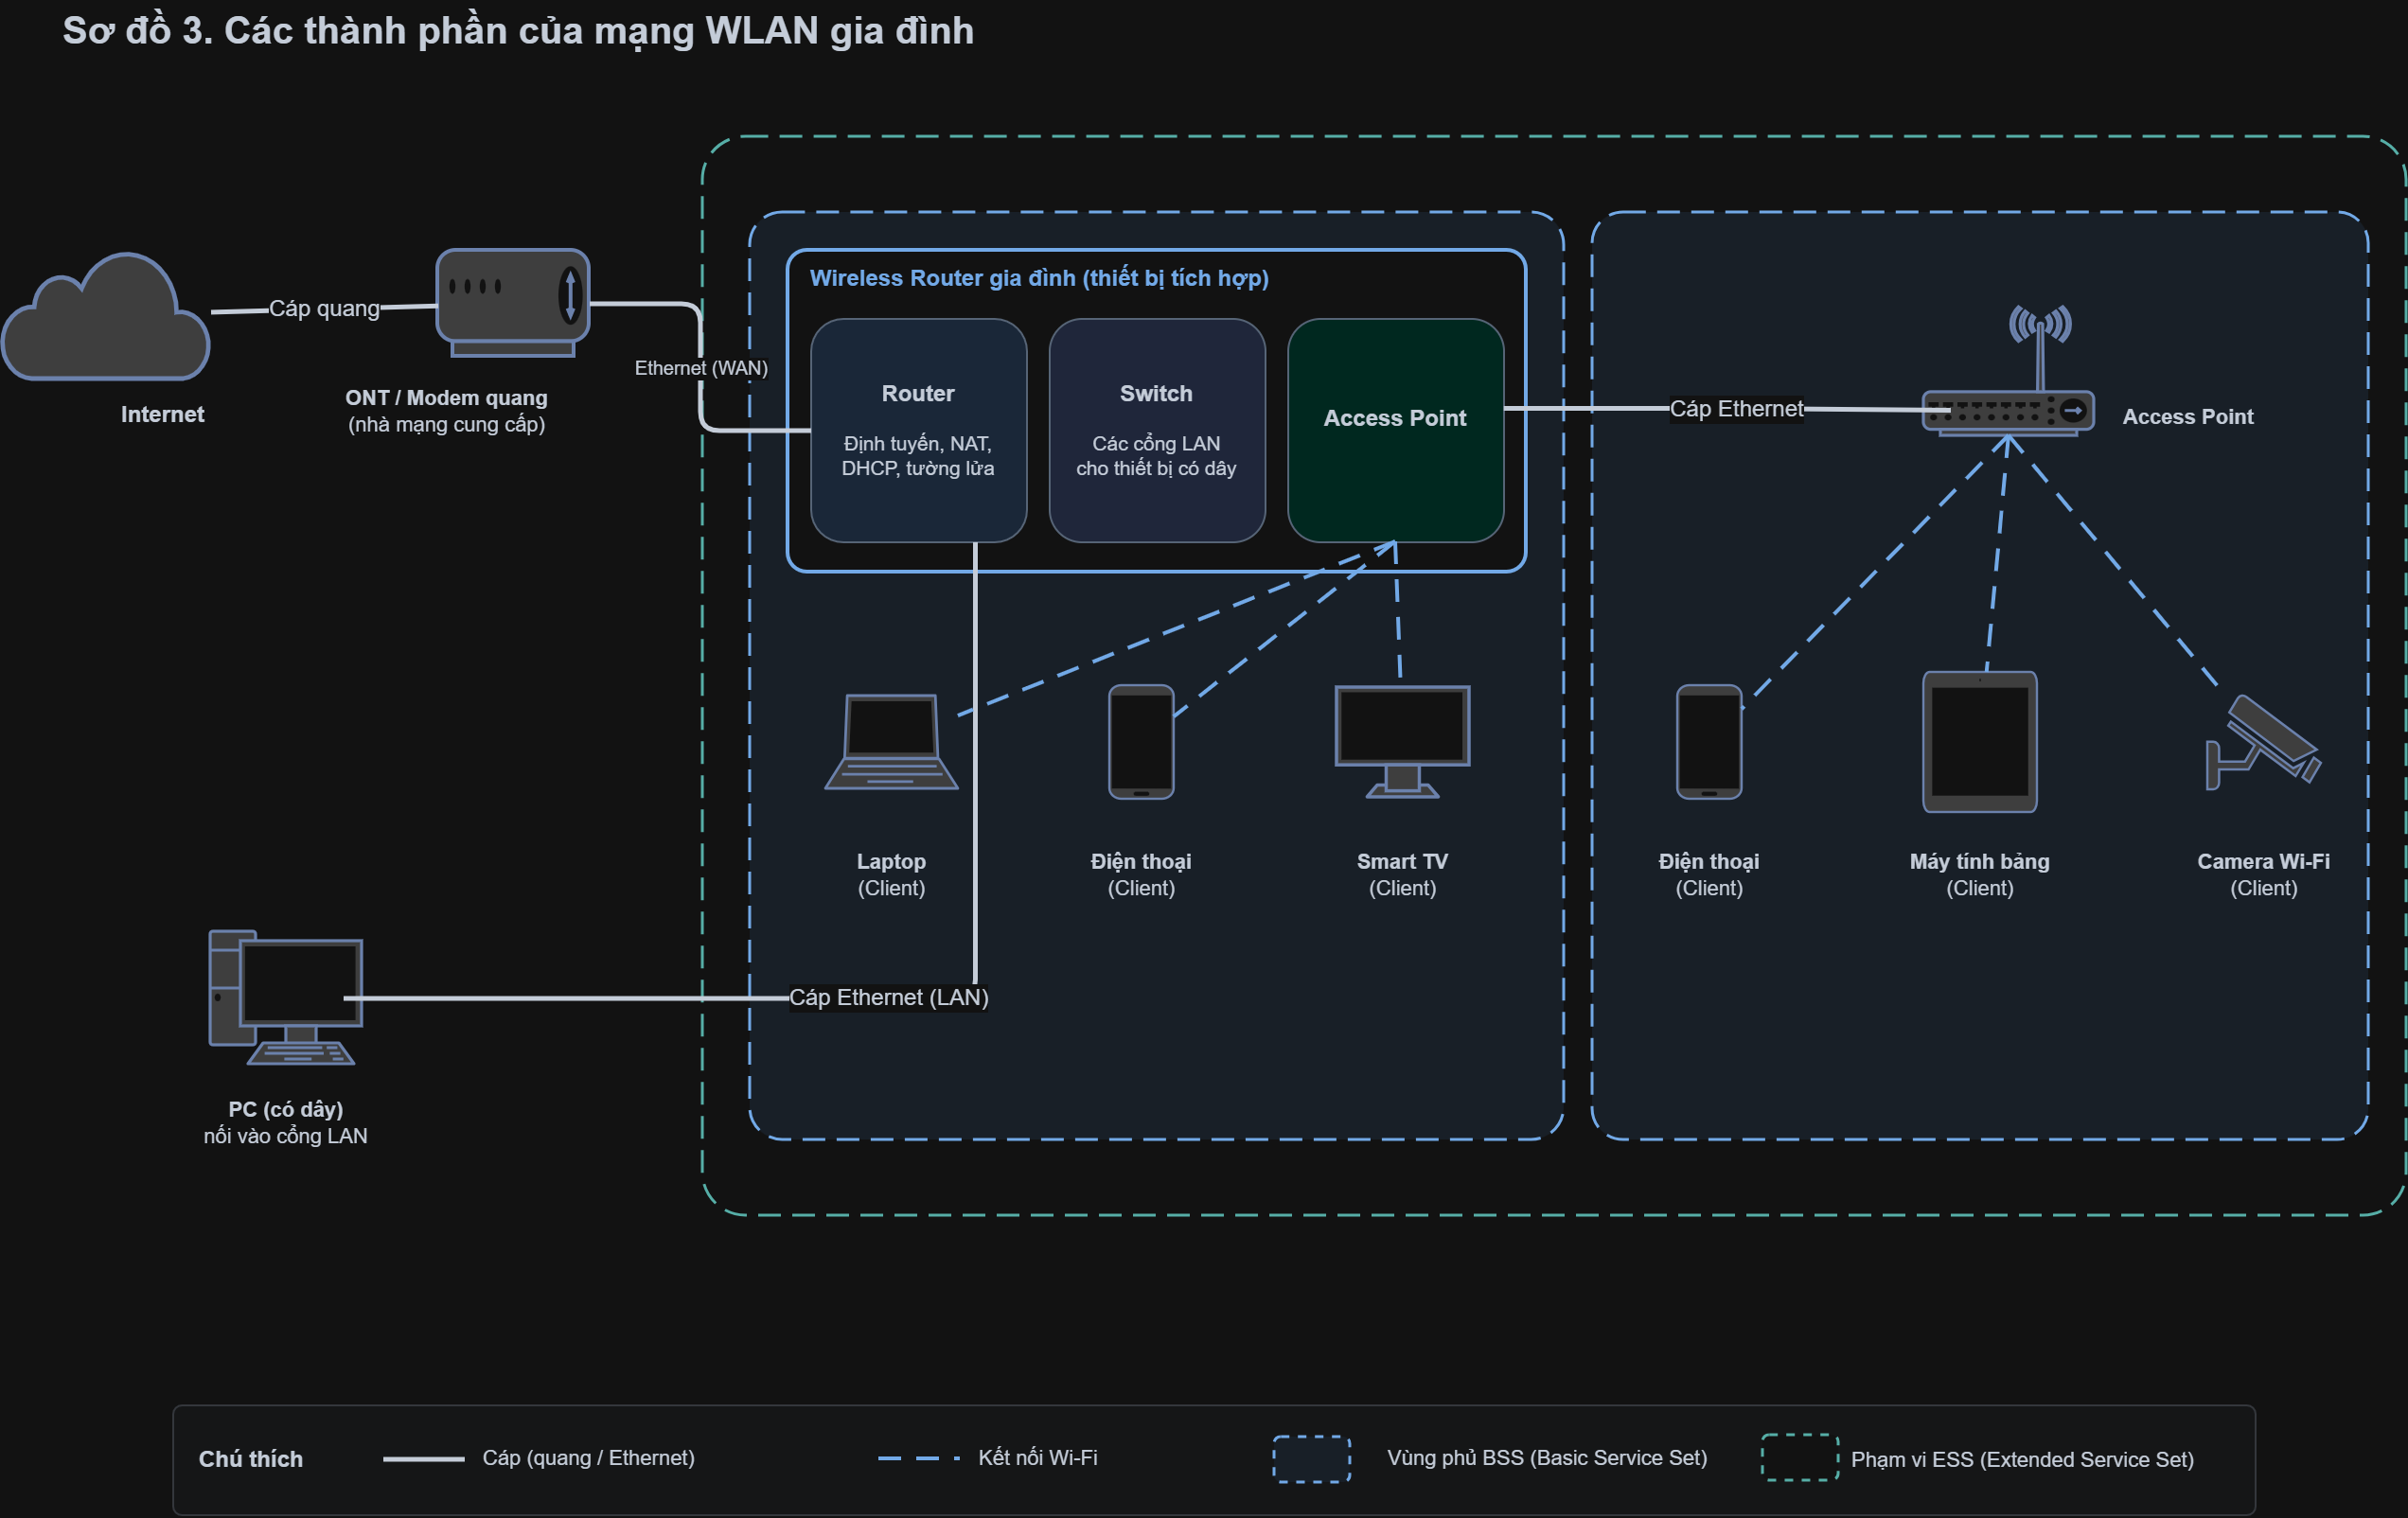
\includegraphics[width=\linewidth]{figures/N09_sodo3_thanhphan.png}
  \caption[Các thành phần của một mạng WLAN gia đình]{Các thành phần của một mạng WLAN gia đình: modem quang, bộ định tuyến
  tích hợp (định tuyến/NAT/DHCP, switch cổng LAN, \ac{ap}), các thiết bị đầu cuối
  không dây và thiết bị có dây; nét đứt thể hiện vùng phủ \ac{bss} và phạm vi
  \ac{ess}.}
  \label{fig:sodo-thanhphan}
\end{figure}

\textbf{Phạm vi định danh: \ac{bss} và \ac{bssid}.} \ac{bss} là đơn vị cấu
thành cơ bản nhất của mạng Wi-Fi theo mô hình hạ tầng: một \ac{ap} duy nhất cùng
toàn bộ thiết bị không dây đang liên kết trực tiếp với \ac{ap} đó. Để phân biệt
các \ac{bss} với nhau, mỗi \ac{bss} mang một mã định danh duy nhất là
\ac{bssid}, và trong mô hình hạ tầng \ac{bssid} chính là địa chỉ MAC vật lý của
giao diện vô tuyến trên \ac{ap}.

\textbf{Mở rộng và chuyển vùng: \ac{ess}.} \ac{ess} là mô hình mở rộng, hình
thành khi nhiều \ac{bss} (nhiều \ac{ap}) được nối với nhau qua \ac{ds} để phủ
sóng một không gian lớn hơn. Mọi \ac{ap} trong cùng một \ac{ess} dùng chung một
\ac{ssid} và cùng cấu hình bảo mật, mặc dù mỗi \ac{ap} vẫn sở hữu \ac{bssid}
riêng. Nhờ đó thiết bị đầu cuối có thể di chuyển liên tục giữa các vùng phủ sóng
mà không bị ngắt kết nối (roaming). Cần lưu ý rằng \ac{ess} truyền thống không
có cơ chế chuyển vùng nhanh, nên việc chọn \ac{ap} nào để liên kết là do chính
thiết bị của người dùng quyết định dựa trên cường độ tín hiệu; các tiêu chuẩn
802.11k/v/r sau này mới bổ sung cơ chế hỗ trợ chuyển vùng nhanh và cân bằng tải.

\subsubsection{Mô hình tùy biến (Ad-hoc / IBSS)}

Mô hình Ad-hoc là một mạng lưới phi tập trung: không có thiết bị nào làm chủ và
tất cả các nút đều bình đẳng. Thành phần thiết bị chỉ gồm các nút không dây
(\emph{wireless nodes}) -- chính là các thiết bị đầu cuối như máy tính xách tay
hay máy tính để bàn gắn card/USB Wi-Fi -- và không có điểm truy cập trung tâm.
Trong mạng nhiều chặng, các nút có thể được cấu hình thêm để chuyển tiếp gói tin
và thực hiện định tuyến; IBSS cơ bản chỉ cung cấp liên lạc trực tiếp giữa các
nút trong cùng vùng phủ sóng. Hình~\ref{fig:sodo-adhoc} mô tả dạng triển khai hai nút mà nhóm dùng để
kiểm chứng mô hình này (xem Mục~\ref{sec:adhoc-config} và
Mục~\ref{sec:experiment}).

\begin{figure}[htbp]
  \centering
  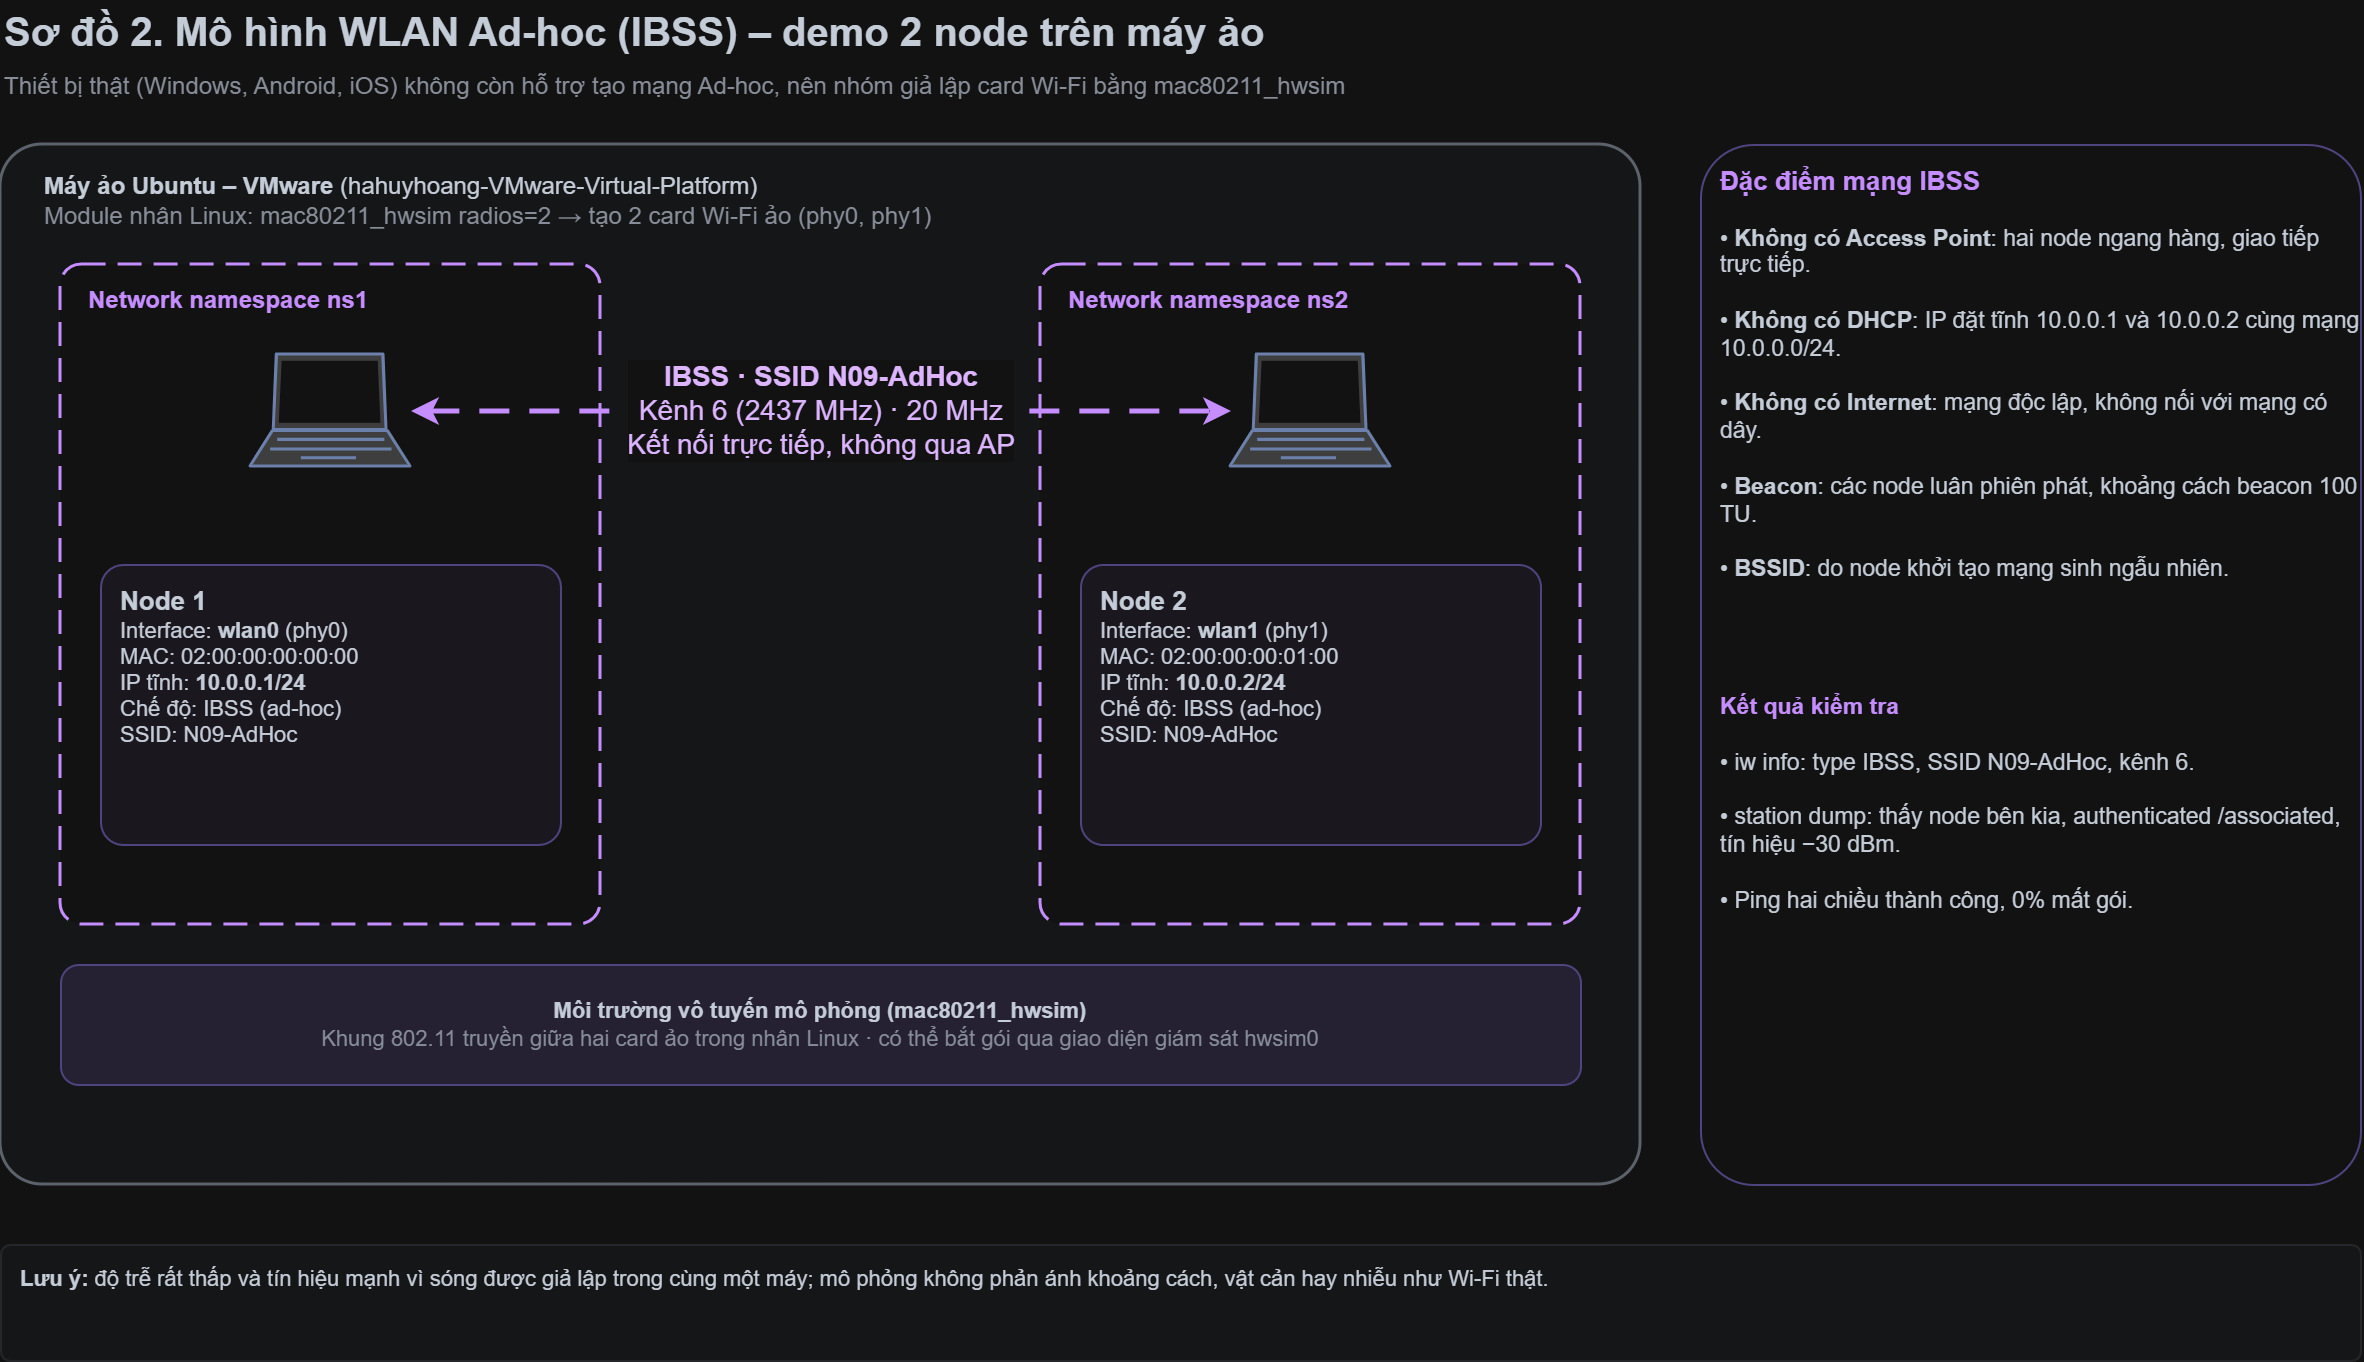
\includegraphics[width=\linewidth]{figures/N09_sodo2_adhoc.png}
  \caption[Sơ đồ mô hình Ad-hoc (IBSS) hai nút trên máy ảo]{Sơ đồ mô hình Ad-hoc (\ac{ibss}) hai nút trên máy ảo: hai card Wi-Fi ảo
  \texttt{phy0}, \texttt{phy1} được tách vào hai network namespace, cùng tham gia
  \ac{ibss} \texttt{N09-AdHoc} trên kênh~6 và giao tiếp trực tiếp, không qua
  \ac{ap}.}
  \label{fig:sodo-adhoc}
\end{figure}

\textbf{Định danh trong \ac{ibss}.} Ở mạng hạ tầng (\ac{bss}), \ac{bssid} là địa
chỉ MAC thật của \ac{ap}. Ở mạng Ad-hoc, vì không có \ac{ap}, nút đầu tiên khởi
tạo mạng sẽ tự sinh một địa chỉ MAC ảo ngẫu nhiên để làm \ac{bssid}; các nút
tham gia sau đó cùng dùng chung mã \ac{bssid} ảo này để nhận diện nhau.

\textbf{Duy trì mạng bằng beacon phân tán.} Trong \ac{bss}, \ac{ap} liên tục
phát khung beacon để thông báo mạng còn tồn tại. Trong \ac{ibss}, do các nút
bình đẳng, các nút tranh chấp cơ hội phát beacon tại mỗi thời điểm phát mục tiêu;
chu kỳ thường dùng là 100~TU. Nhờ đó không cần một nguồn
phát duy nhất mà mạng vẫn được duy trì.

\textbf{Tính cô lập.} \ac{ibss} là một ``hòn đảo'' độc lập: mặc định nó không
thể giao tiếp với hệ thống mạng có dây bên ngoài và không có kết nối Internet.
Đây là khác biệt bản chất so với mô hình hạ tầng, nơi \ac{ds} và bộ định tuyến
biên mở đường ra mạng ngoài.

\textbf{Giới hạn công nghệ.} Mạng Ad-hoc hoạt động ổn định nhất trên các chuẩn
Wi-Fi cũ là 802.11b, 802.11g và 802.11n ở băng tần 2,4~GHz. Về bảo mật, phần
lớn triển khai \ac{ibss} trên hệ điều hành phổ thông chỉ hỗ trợ mã hóa
\ac{wep} -- loại mã hóa đã bị chứng minh có thể bị phá trong vài phút -- hoặc
buộc phải để mạng mở không mật khẩu; do đó mô hình này không phù hợp cho dữ liệu
nhạy cảm. Ngoài ra, hiệu năng suy giảm rõ rệt khi số nút tăng, vì toàn bộ việc
điều phối kênh diễn ra phân tán và không có thiết bị nào quản lý tài nguyên vô
tuyến.

\textbf{Tiến hóa của mô hình.} Trên các thiết bị hằng ngày như điện thoại, máy
tính xách tay hay máy tính cá nhân, chế độ Ad-hoc đã được thay thế bằng
Wi-Fi Direct. Đối với các mạng như MANET, VANET hay FANET, đây là phiên bản
tiến hóa cao cấp nhất của mạng Ad-hoc: chúng vẫn thuần túy ngang hàng nhưng được
bổ sung các giao thức định tuyến (routing protocol) khá phức tạp ở tầng mạng
(lớp~3) để chuyển tiếp gói qua nhiều chặng, và vẫn đang được sử dụng trong những
lĩnh vực chuyên biệt như cứu hộ -- cứu nạn, giao thông thông minh hay thiết bị
bay không người lái.

\subsubsection{Mô hình hạ tầng do nhóm triển khai trên thiết bị thật}

Để phần lý thuyết gắn với thực nghiệm, nhóm triển khai mô hình hạ tầng trên một
bộ định tuyến thật là TP-Link Archer C20 v5 cài phần mềm OpenWrt, tên thiết bị
\texttt{N09-Router}, với địa chỉ quản trị \texttt{192.168.1.1}. Router có hai bộ
phát: bộ 2,4~GHz dùng chip MediaTek MT7628 theo chuẩn 802.11b/g/n và bộ 5~GHz
dùng chip MT7610E theo chuẩn 802.11ac.

Hình~\ref{fig:sodo-n09} là sơ đồ mạng mà nhóm đã dựng và đo được. Hai điểm đáng
chú ý về mặt lý thuyết:

\begin{itemize}[leftmargin=*]
  \item Mỗi bộ phát tạo một \ac{bss} riêng nên có \ac{bssid} riêng: bộ 2,4~GHz
    dùng \texttt{B0:95:75:9F:1C:A3} (kênh~6, 2,437~GHz, độ rộng 20~MHz), bộ
    5~GHz dùng \texttt{B0:95:75:9F:1C:A2} (kênh~36, 5,180~GHz, 802.11ac,
    WPA2-PSK/CCMP). Hai \ac{bssid} chỉ khác nhau một bit, phản ánh việc hai giao
    diện vô tuyến nằm trên cùng một thiết bị.
  \item Cả ba thiết bị di động trong mạng đều tự chọn liên kết vào \ac{bss}
    5~GHz, còn \ac{bss} 2,4~GHz không có trạm nào. Đây là minh chứng thực tế cho
    nhận định ở Mục~\ref{sec:arch}: việc chọn \ac{ap} và băng tần là do thiết bị
    đầu cuối quyết định, thường theo cường độ tín hiệu và băng thông hỗ trợ.
\end{itemize}

\begin{figure}[htbp]
  \centering
  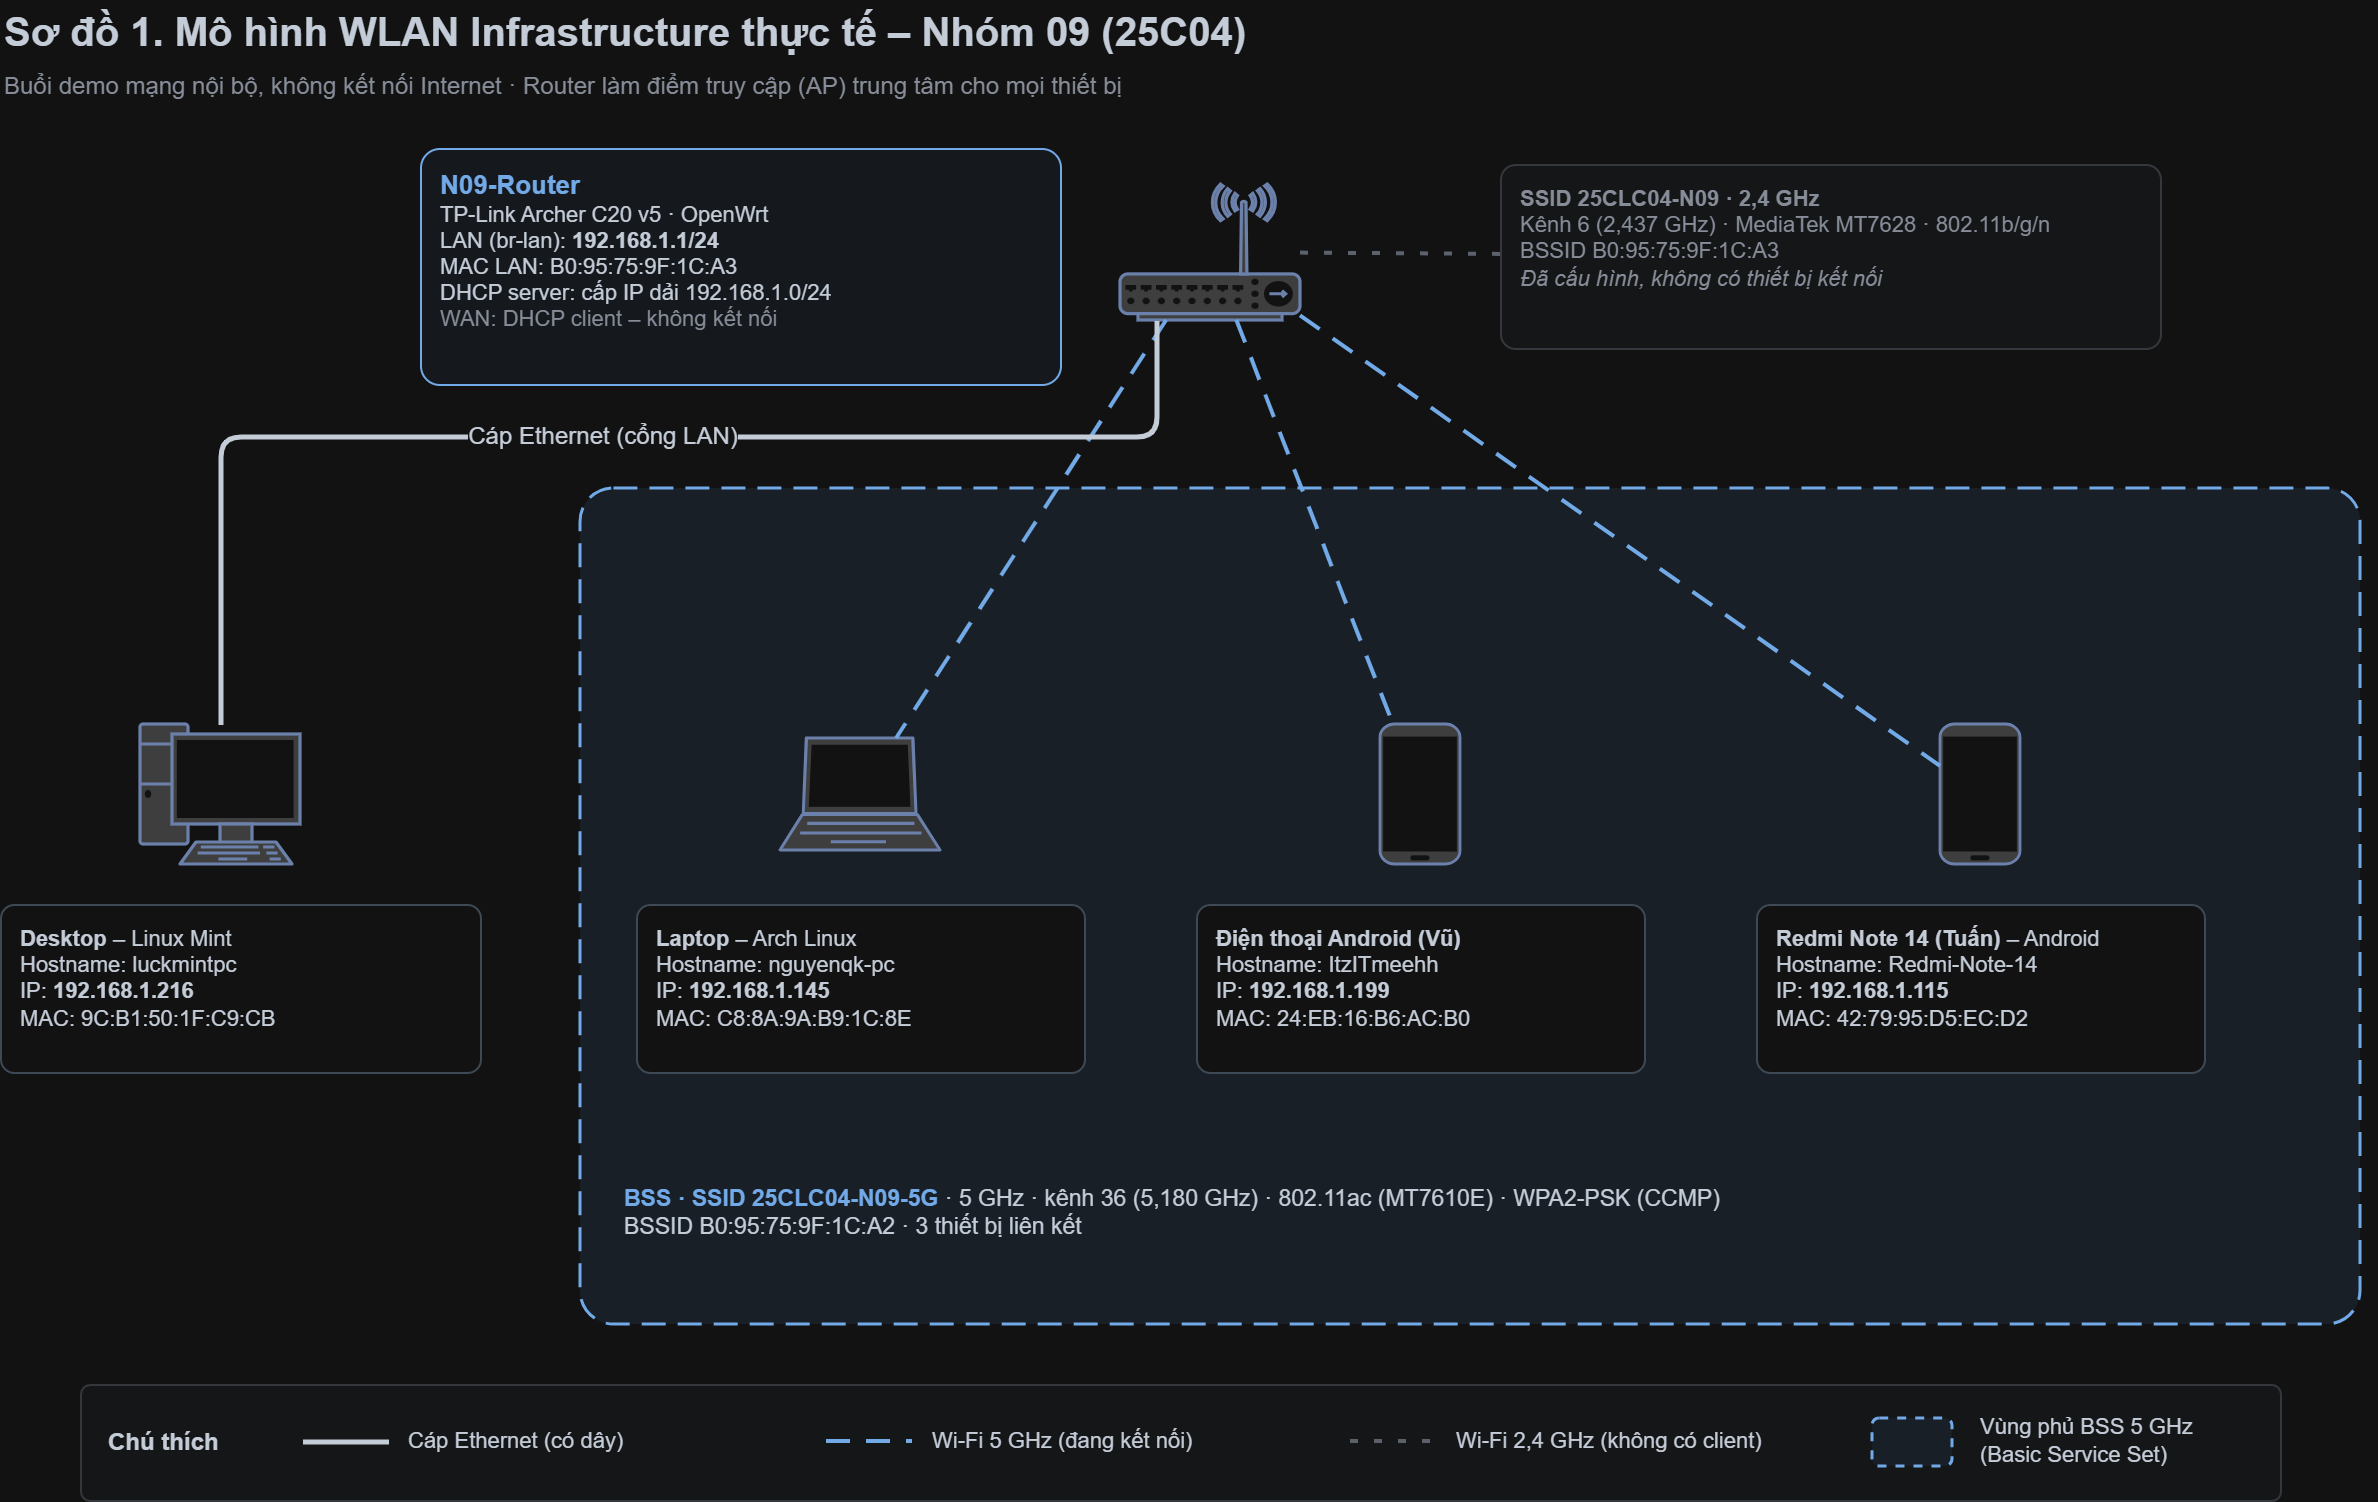
\includegraphics[width=\linewidth]{figures/N09_sodo1_infrastructure.png}
  \caption[Sơ đồ mô hình WLAN Infrastructure thực tế của nhóm]{Sơ đồ mô hình WLAN Infrastructure thực tế của nhóm: bộ định tuyến
  N09-Router (TP-Link Archer C20 v5, OpenWrt) làm \ac{ap} trung tâm, một máy bàn
  nối bằng cáp Ethernet vào cổng LAN và ba thiết bị di động liên kết vào
  \ac{bss} 5~GHz.}
  \label{fig:sodo-n09}
\end{figure}

\subsubsection{Đối chiếu chi tiết giữa hai mô hình}

Bảng~\ref{tab:infra-adhoc-detail} hệ thống hóa các khác biệt ở mức kiến trúc,
định danh, vận hành và bảo mật. Bảng này bổ sung cho bảng so sánh tổng quát
(Bảng~\ref{tab:infra-vs-adhoc}) bằng các tiêu chí cụ thể đã được kiểm chứng
trong quá trình thực nghiệm.

\begin{table}[htbp]
  \centering\footnotesize
  \caption{Đối chiếu chi tiết giữa mô hình hạ tầng (Infrastructure) và mô hình
  tùy biến (Ad-hoc / IBSS).}
  \label{tab:infra-adhoc-detail}
  \begin{tabularx}{\linewidth}{@{} L{0.75} L{1.15} L{1.1} @{}}
    \toprule
    \textbf{Tiêu chí} & \textbf{Mô hình hạ tầng (Infrastructure)} & \textbf{Mô hình tùy biến (Ad-hoc / \ac{ibss})} \\
    \midrule
    Thiết bị trung tâm & Bắt buộc có \ac{ap} hoặc bộ định tuyến không dây đảm
      nhiệm phát sóng và chuyển tiếp & Không có; các \ac{sta} hoàn toàn ngang
      hàng và tự chuyển tiếp cho nhau \\
    Đơn vị cấu thành & \ac{bss} (một \ac{ap}) mang \ac{bssid} riêng; nhiều
      \ac{bss} ghép thành \ac{ess} & \ac{ibss}: một nhóm nút độc lập, không có
      \ac{ap} \\
    Nguồn \ac{bssid} & Địa chỉ MAC vật lý của giao diện vô tuyến trên \ac{ap} &
      Địa chỉ MAC ảo sinh ngẫu nhiên bởi nút khởi tạo mạng, các nút khác dùng
      chung \\
    Phát beacon & \ac{ap} phát định kỳ, một nguồn phát duy nhất & Các nút phân
      tán cơ hội phát beacon; 100~TU là chu kỳ thường dùng \\
    Điều phối truy cập kênh & \ac{ap} giữ vai trò chủ; có thể hỗ trợ DCF hoặc
      PCF/HCCA & Phân tán hoàn toàn, chỉ hoạt động theo DCF (\ac{csmaca}) \\
    Cấp phát địa chỉ IP & Máy chủ DHCP tập trung trên \ac{ds} & Gán tĩnh thủ
      công, không có máy chủ DHCP \\
    Kết nối ra mạng ngoài & Có, qua \ac{ds} và bộ định tuyến biên & Mặc định
      không có; mạng bị cô lập với \ac{lan} có dây và Internet \\
    Mở rộng và chuyển vùng & Tốt; thêm \ac{ap} cùng \ac{ssid} là mở rộng
      \ac{ess}, hỗ trợ chuyển vùng & Kém; mọi nút phải trùng \ac{ssid} và trùng
      kênh, không có chuyển vùng; hiệu năng giảm khi số nút tăng \\
    Bảo mật & Đầy đủ; hỗ trợ WPA2/WPA3, 802.1X/\ac{radius} cho doanh nghiệp &
      Hạn chế; thực tế chỉ \ac{wep} hoặc mạng mở, không có WPA2/WPA3 \\
    Chuẩn và băng tần & Mọi thế hệ 802.11 và mọi băng tần được cấp phép & Ổn
      định nhất trên 802.11b/g/n, băng tần 2,4~GHz \\
    Hỗ trợ trên hệ điều hành phổ thông & Mặc định trên Windows, Android, iOS và
      macOS & Phụ thuộc hệ điều hành, driver và phần cứng; Linux thường cung cấp
      công cụ cấu hình IBSS đầy đủ hơn \\
    Ứng dụng thực tế & Gia đình, văn phòng, trường học, doanh nghiệp & Chia sẻ
      dữ liệu tạm thời, cứu nạn khẩn cấp, mạng cảm biến; nay chủ yếu được thay
      bằng Wi-Fi Direct \\
    \bottomrule
  \end{tabularx}
\end{table}

Từ đối chiếu trên có thể rút ra định hướng lựa chọn mô hình: hiệu năng, khả năng
mở rộng, kết nối Internet và bảo mật hiện đại là những lý do khiến mô hình hạ
tầng vẫn là mặc định cho mọi nhu cầu khai thác thực tế; mô hình Ad-hoc chỉ còn
giá trị ở những tình huống không thể dựng hạ tầng, hoặc trong các dạng tiến hóa
đa chặng phục vụ mục đích chuyên biệt. Chính vì giới hạn về bảo mật và khả năng
kết nối, phần Ad-hoc của báo cáo chỉ dùng chế độ \ac{ibss} để kiểm chứng nguyên
lý ngang hàng ở mức hai nút trên nền Linux
(Mục~\ref{sec:adhoc-config} và Mục~\ref{sec:experiment}), trong khi mọi nội dung
về bảo mật, cấp phát địa chỉ và kết nối Internet được kiểm chứng trên mô hình hạ
tầng với router thật.

\endgroup

\section{Giải pháp kết nối Laptop, Desktop và Smartphone}
\label{sec:device-connectivity}

Trong mô hình Infrastructure, các thiết bị đầu cuối kết nối tới cùng điểm truy
cập (access point -- AP) bằng định danh mạng (SSID) và phương thức xác thực
được cấu hình thống nhất. Sau khi liên kết lớp vô tuyến, thiết bị nhận cấu hình
địa chỉ IP tự động qua DHCP hoặc sử dụng cấu hình tĩnh phù hợp với mạng.

\subsection{Máy tính xách tay (Laptop)}
Kiểm tra bộ điều hợp Wi-Fi đã bật và hỗ trợ băng tần, chuẩn bảo mật của AP. Chọn
SSID, nhập thông tin xác thực, xác nhận địa chỉ IP, cổng mặc định và máy chủ DNS;
kiểm tra kết nối mạng nội bộ và Internet.

\subsection{Máy tính để bàn (Desktop)}
Máy tính để bàn có thể dùng card Wi-Fi PCIe/USB hoặc kết nối Ethernet tới LAN.
Nếu dùng Wi-Fi, thực hiện ghép nối như Laptop; nếu dùng Ethernet, bảo đảm cổng
LAN của router/AP hoạt động và cấu hình IP tương thích với cùng mạng con.

\subsection{Điện thoại thông minh (Smartphone)}
Trên Android hoặc iOS, bật Wi-Fi, chọn SSID và xác thực theo chính sách của
mạng. Với mạng doanh nghiệp, nhập thông tin 802.1X theo hướng dẫn quản trị viên.
Không chia sẻ mật khẩu qua kênh không an toàn; ưu tiên WPA2-AES hoặc WPA3 khi
thiết bị hỗ trợ.

\subsection{Kết nối ngang hàng Ad-hoc}
Trong mạng Ad-hoc (IBSS), các trạm tương thích kết nối trực tiếp, không qua AP.
Khả năng hỗ trợ tùy hệ điều hành, trình điều khiển và phần cứng; Wi-Fi Direct
là một cơ chế ngang hàng phổ biến trên thiết bị hiện đại nhưng không đồng nhất
hoàn toàn với IBSS.

\begingroup
% Kiểu cột L cho tabularx (khai báo trong nhóm riêng, theo quy ước của báo cáo).
\newcolumntype{L}[1]{>{\hsize=#1\hsize\raggedright\arraybackslash}X}

\section{Hướng dẫn cấu hình bộ định tuyến và các thiết bị}
\label{sec:configuration-guide}

Phần này ghi lại quy trình cấu hình đã thực hiện trên thiết bị thật của nhóm, kèm
các giá trị thực tế đọc được trên giao diện quản trị. Tên menu tương ứng với bản
OpenWrt cài trên bộ định tuyến; với phần sụn của nhà sản xuất khác, tên mục có thể khác
nhưng nguyên tắc cấu hình không đổi. Không đăng tải mật khẩu quản trị hoặc mật
khẩu Wi-Fi thật vào báo cáo.

\subsection{Thiết bị và thông số thực tế}
\label{subsec:thiet-bi-thuc-te}

\begin{table}[htbp]
  \centering\footnotesize
  \caption{Thông số thiết bị và cấu hình mạng đã thiết lập trên N09-Router.}
  \label{tab:cauhinh-thucte}
  \begin{tabularx}{\linewidth}{@{} L{0.62} L{1.38} @{}}
    \toprule
    \textbf{Hạng mục} & \textbf{Giá trị thực tế} \\
    \midrule
    Mẫu thiết bị / phần mềm & TP-Link Archer C20 v5, phần sụn OpenWrt, giao diện quản trị
      LuCI \\
    Tên thiết bị & \texttt{N09-Router} \\
    Địa chỉ quản trị & \texttt{192.168.1.1} (giao diện \texttt{br-lan}),
      \texttt{192.168.1.0/24} \\
    MAC giao diện LAN & \texttt{B0:95:75:9F:1C:A3} \\
    Bộ phát 2,4~GHz & MediaTek MT7628, 802.11b/g/n, kênh~6 (2,437~GHz), rộng
      20~MHz, mã quốc gia VN \\
    \ac{ssid} 2,4~GHz & \texttt{25CLC04-N09}, WPA2-PSK, mã hóa CCMP (AES) \\
    Bộ phát 5~GHz & MediaTek MT7610E, 802.11ac, kênh~36 (5,180~GHz), rộng
      80~MHz \\
    \ac{ssid} 5~GHz & \texttt{25CLC04-N09-5G}, WPA2-PSK, mã hóa CCMP; \ac{bssid}
      \texttt{B0:95:75:9F:1C:A2} \\
    Mạng khách & \texttt{25CLC04-N09-Guest}, dải \texttt{192.168.20.0/24}, cổng
      \texttt{192.168.20.1}, DHCP riêng, vùng tường lửa riêng \\
    Cấp địa chỉ & DHCP trên \ac{lan}, thời hạn thuê 12~h; có đặt IP tĩnh theo MAC
      cho máy bàn (\texttt{192.168.1.50}) \\
    Cổng WAN & Chế độ DHCP client; trong sơ đồ demo cuối cùng cổng WAN không nối
      ra Internet \\
    \bottomrule
  \end{tabularx}
\end{table}

\subsection{Cấu hình cơ bản trên giao diện LuCI}
\begin{enumerate}[leftmargin=*]
  \item \textbf{Đăng nhập và đặt mật khẩu quản trị.} Máy quản trị nối vào cổng
    LAN (hoặc vào Wi-Fi tạm), mở \texttt{http://192.168.1.1}. Router mới ở trạng
    thái chưa có mật khẩu nên hiện cảnh báo; đặt mật khẩu cho tài khoản
    \texttt{root} ngay từ lần đăng nhập đầu tiên. Đây là bước bắt buộc vì ai cắm
    được dây vào cổng LAN cũng có thể thay đổi toàn bộ cấu hình.
  \item \textbf{Đặt tên thiết bị và múi giờ.} Vào \emph{System $\rightarrow$
    System}, đổi Hostname thành \texttt{N09-Router}, chọn múi giờ
    \emph{Asia/Ho\_Chi\_Minh} rồi đồng bộ giờ với máy quản trị. Việc đặt đúng
    múi giờ là điều kiện để các luật chặn theo khung giờ ở
    Mục~\ref{subsec:cauhinh-nangcao} hoạt động đúng.
  \item \textbf{Cấu hình \ac{lan} và DHCP.} Vào \emph{Network $\rightarrow$
    Interfaces}, đặt địa chỉ \ac{lan} \texttt{192.168.1.1/24} và bật máy chủ DHCP
    cho dải này. Cổng WAN để ở chế độ DHCP client để nhận địa chỉ từ modem hoặc
    router phía trên khi cần nối Internet.
  \item \textbf{Cấu hình Wi-Fi 2,4~GHz.} Vào \emph{Network $\rightarrow$
    Wireless}, mở thiết bị MT7628: chọn Country Code \texttt{VN}, Mode \texttt{N},
    Channel \texttt{6}, Width \texttt{20~MHz}; phần Interface đặt ESSID
    \texttt{25CLC04-N09}, Mode \emph{Access Point}, Network \texttt{lan}.
  \item \textbf{Cấu hình Wi-Fi 5~GHz.} Mở thiết bị MT7610E: Country Code
    \texttt{VN}, Mode \texttt{AC}, Channel \texttt{36}, Width \texttt{80~MHz};
    ESSID \texttt{25CLC04-N09-5G}.
  \item \textbf{Cấu hình bảo mật.} Ở tab \emph{Wireless Security} của mỗi mạng,
    chọn Encryption WPA2-PSK, Cipher \emph{Force CCMP (AES)} và đặt khóa dài, khó
    đoán. Sau khi bấm \emph{Save \& Apply}, trang Wireless hiển thị hai mạng đang
    phát, mỗi mạng kèm một \ac{bssid} riêng -- đúng với mô tả lý thuyết về
    \ac{bss} và \ac{bssid}.
\end{enumerate}

\subsection{Các chức năng quản lý đã cấu hình và thử}
\label{subsec:cauhinh-nangcao}

Các chức năng dưới đây được thiết lập trên N09-Router và được quay lại trong
video minh chứng (Mục~\ref{sec:video}). Cột ``Kết quả quan sát'' chỉ ghi những gì
thực sự thấy trên màn hình, không suy diễn thêm.

\begin{table}[htbp]
  \centering\footnotesize
  \caption{Các chức năng quản lý đã cấu hình trên router và kết quả quan sát.}
  \label{tab:chucnang-router}
  \begin{tabularx}{\linewidth}{@{} L{0.7} L{1.1} L{1.2} @{}}
    \toprule
    \textbf{Chức năng} & \textbf{Đường dẫn cấu hình} & \textbf{Kết quả quan sát} \\
    \midrule
    Ẩn tên mạng & Wireless $\rightarrow$ Hide ESSID & Mạng 2,4~GHz biến mất khỏi
      danh sách quét của thiết bị thử, mạng 5~GHz vẫn hiện; bật lại thì mạng hiện
      lại bình thường \\
    Mạng khách tách riêng & Interfaces + Wireless + Firewall zone
      \texttt{guest} & Thiết bị thử nhận địa chỉ trong dải
      \texttt{192.168.20.0/24}, ra Internet bình thường nhưng không mở được trang
      quản trị \texttt{192.168.1.1} \\
    Lọc địa chỉ MAC & Wireless $\rightarrow$ MAC-Filter & Thêm MAC thiết bị thử
      vào danh sách chặn: thiết bị bị ngắt và không kết nối lại được dù đúng mật
      khẩu; tắt lọc thì vào lại được \\
    Cấp IP tĩnh theo MAC & DHCP and DNS $\rightarrow$ Static Leases & Máy bàn tắt
      rồi bật Wi-Fi, nhận đúng \texttt{192.168.1.50} như đã gán \\
    Chặn tên miền & DHCP and DNS $\rightarrow$ DNS Records & Trỏ
      \texttt{vnexpress.net} và \texttt{www.vnexpress.net} về \texttt{0.0.0.0}:
      trình duyệt không mở được trang này, các trang khác vẫn bình thường; xóa
      luật thì truy cập lại được \\
    Giới hạn giờ truy cập & Firewall $\rightarrow$ Traffic Rules + Time
      Restrictions & Luật chặn theo MAC nguồn ra vùng \texttt{wan}: thiết bị vẫn
      báo có Wi-Fi nhưng không mở được trang web; tắt luật thì vào lại được \\
    Chuyển tiếp cổng & Firewall $\rightarrow$ Port Forwards & Từ ngoài mạng, mở
      địa chỉ WAN cổng 8080 truy cập được dịch vụ trên máy bàn; xóa luật thì
      không còn truy cập \\
    NAT và chẩn đoán & Firewall (Masquerading), Network $\rightarrow$
      Diagnostics & Vùng \texttt{wan} bật Masquerading (NAT); Traceroute tới
      \texttt{8.8.8.8} cho thấy gói tin đi qua router của mạng nhà trước khi ra
      nhà cung cấp dịch vụ \\
    Sao lưu cấu hình & System $\rightarrow$ Backup / Flash Firmware & Tạo được
      tệp lưu trữ cấu hình để phục hồi khi cần \\
    \bottomrule
  \end{tabularx}
\end{table}

\subsection{Kết nối Laptop, Desktop và Smartphone}
Máy bàn (Desktop) được nối bằng cáp Ethernet vào cổng LAN và cũng đã được thử
kết nối bằng Wi-Fi để chứng minh card không dây hoạt động. Laptop và điện thoại
được kết nối lần lượt vào mạng của nhóm; với thiết bị di động và Windows cần tắt
tính năng \emph{địa chỉ MAC ngẫu nhiên} cho mạng này, nếu không địa chỉ MAC hiện
trên router sẽ khác MAC thật và các luật lọc MAC ở trên sẽ không chạy đúng.

Trên mỗi thiết bị, sau khi kết nối cần kiểm tra: địa chỉ IP nhận được, cổng mặc
định (phải là \texttt{192.168.1.1}), băng tần và kênh đang dùng, kiểu bảo mật, và
khả năng liên lạc với router cũng như với thiết bị khác trong mạng. Kết quả đo
cụ thể được trình bày ở Mục~\ref{sec:experiment}.

\subsection{Thiết lập và kiểm chứng mạng Ad-hoc (IBSS) trên nền Linux}
\label{sec:adhoc-config}

Trước khi cấu hình, cần xác nhận nền tảng có hỗ trợ chế độ ngang hàng hay không.
Trên Windows~11, lệnh \texttt{netsh wlan show drivers} trả về dòng
\emph{Hosted network supported: No}, nghĩa là hệ điều hành không còn hỗ trợ chế
độ Ad-hoc (minh chứng tại Hình~\ref{fig:win-hosted}); Android và macOS cũng
không hỗ trợ. Vì vậy quy trình dưới đây được thực hiện trên Linux, sử dụng module
\texttt{mac80211\_hwsim} để mô phỏng phần cứng Wi-Fi và hai network namespace để
tách hai nút thành hai máy độc lập. Không được gọi nhầm chế độ hotspot hay
Wi-Fi Direct là \ac{ibss}.

\begin{enumerate}[leftmargin=*]
  \item \textbf{Kiểm tra nền tảng và tạo card Wi-Fi ảo.} Nạp module mô phỏng với
    hai radio: \texttt{sudo modprobe mac80211\_hwsim radios=2}, sau đó kiểm tra
    bằng \texttt{iw dev}. Mỗi radio tương ứng một giao diện (\texttt{wlan0},
    \texttt{wlan1}) có kênh, công suất phát và thuộc tính phần cứng riêng.
    Giao diện \texttt{P2P-device} do trình điều khiển tự tạo không ảnh hưởng
    đến kết nối Ad-hoc.

  \item \textbf{Tách mỗi radio vào một network namespace.} Nếu hai giao diện nằm
    chung một hệ thống, chúng dùng chung bảng định tuyến nên Linux coi cả hai
    địa chỉ IP là của chính nó và chuyển gói qua loopback, khiến lưu lượng không
    đi qua ``sóng'' vô tuyến ảo. Thực hiện:
    \texttt{sudo ip netns add ns1} và \texttt{sudo ip netns add ns2};
    \texttt{sudo iw phy phy0 set netns name ns1};
    \texttt{sudo iw phy phy1 set netns name ns2}. Kiểm tra lại bằng
    \texttt{sudo ip netns exec ns1 iw dev} và
    \texttt{sudo ip netns exec ns2 iw dev}.

  \item \textbf{Chuyển giao diện sang chế độ \ac{ibss} và tham gia mạng.} Với
    mỗi nút, hạ giao diện xuống trước khi đổi chế độ (nếu không, nhân hệ điều
    hành báo lỗi \emph{Device or resource busy}). Với Node~1 trong \texttt{ns1}:
    \texttt{sudo ip netns exec ns1 ip link set wlan0 down};
    \texttt{sudo ip netns exec ns1 iw dev wlan0 set type ibss};
    \texttt{sudo ip netns exec ns1 ip link set wlan0 up};
    \texttt{sudo ip netns exec ns1 iw dev wlan0 ibss join N09-AdHoc 2437};
    \texttt{sudo ip netns exec ns1 ip addr add 10.0.0.1/24 dev wlan0}. Tham số
    \texttt{N09-AdHoc} là \ac{ssid} của mạng và mọi nút phải trùng;
    \texttt{2437} là tần số tính bằng MHz, tương ứng kênh~6 của băng tần
    2,4~GHz và cũng phải trùng giữa các nút. Node~2 thực hiện tương tự với
    \texttt{ns2}, \texttt{wlan1} và địa chỉ \texttt{10.0.0.2/24}. Mọi lệnh đều
    chạy trong namespace tương ứng thông qua
    \texttt{sudo ip netns exec <namespace>}.

  \item \textbf{Kiểm tra liên kết ở tầng 802.11.} Dùng
    \texttt{iw dev wlan0 info} để xác nhận \texttt{type IBSS}, \ac{ssid},
    kênh và tần số; dùng \texttt{iw dev wlan0 station dump} để xem danh sách nút
    lân cận đã phát hiện. Nếu thấy địa chỉ MAC của nút còn lại ở trạng thái
    \emph{authorized} và \emph{associated}, hai nút đã nhận ra nhau.

  \item \textbf{Kiểm tra liên lạc ở tầng mạng.} Chạy
    \texttt{ping -c 4 10.0.0.2} từ Node~1 và chiều ngược lại từ Node~2. Gói tin
    được đóng khung 802.11, truyền qua ``sóng ảo'' của \texttt{hwsim} tới giao
    diện của nút kia. Kết quả đạt yêu cầu khi cả hai chiều đều nhận đủ 4/4 phản
    hồi và tỉ lệ mất gói bằng 0\,\%.

  \item \textbf{Ghi nhận và dọn dẹp.} Lưu ảnh chụp màn hình từng bước vào phần
    minh chứng (Mục~\ref{sec:evidence}) và ghi lại tham số thực tế. Sau khi kết
    thúc, gỡ namespace và module mô phỏng để trả máy về trạng thái ban đầu.
\end{enumerate}

\subsection{Bảng ghi cấu hình thực tế}
\begin{center}
\begin{tabularx}{\linewidth}{X X X}
  \toprule
  Hạng mục & Giá trị thực tế & Minh chứng/ghi chú \\
  \midrule
  Mẫu thiết bị/bộ định tuyến & TP-Link Archer C20 v5, OpenWrt (LuCI), tên máy
    \texttt{N09-Router} & Bảng~\ref{tab:cauhinh-thucte}; sơ đồ
    Hình~\ref{fig:sodo-n09} \\
  SSID và bảo mật & \texttt{25CLC04-N09} (2,4~GHz) và \texttt{25CLC04-N09-5G}
    (5~GHz), WPA2-PSK/CCMP; mạng khách \texttt{25CLC04-N09-Guest} &
    Bảng~\ref{tab:cauhinh-thucte} \\
  LAN/DHCP & \texttt{192.168.1.1/24}, DHCP thời hạn 12~h, IP tĩnh theo MAC cho
    máy bàn (\texttt{192.168.1.50}) & Bảng~\ref{tab:dhcp-leases} \\
  Laptop/Desktop/Smartphone & 4 thiết bị: máy bàn nối dây, một laptop và hai
    điện thoại Android; cả ba thiết bị không dây đều liên kết \ac{bss} 5~GHz &
    Hình~\ref{fig:sodo-n09}, Bảng~\ref{tab:ping-crosscheck} \\
  Ad-hoc hoặc phương án thay thế & IBSS trên Ubuntu 22.04 LTS (máy ảo VMware),
    \texttt{mac80211\_hwsim radios=2}; \ac{ssid} \texttt{N09-AdHoc}, kênh~6
    (2437~MHz), IP \texttt{10.0.0.1/24} và \texttt{10.0.0.2/24}, mạng mở &
    Hình~\ref{fig:sodo-adhoc}, Hình~\ref{fig:hwsim-radios}--\ref{fig:adhoc-ping};
    Windows~11 không hỗ trợ (Hình~\ref{fig:win-hosted}) \\
  \bottomrule
\end{tabularx}
\end{center}

\endgroup

% =====================================================================
% 06_security.tex
% =====================================================================
\begingroup
\newcolumntype{L}[1]{>{\hsize=#1\hsize\raggedright\arraybackslash}X}

\section{Bảo mật mạng WLAN}
\label{sec:security}

\subsection{Vì sao mạng không dây cần bảo mật mạnh?}

Bất kỳ ai nằm trong vùng phủ sóng vô tuyến đều có thể thu bắt các khung dữ
liệu. Vì vậy, một \ac{wlan} an toàn cần bảo đảm \emph{tính bí mật} (mã hóa),
\emph{tính toàn vẹn} (phát hiện sửa đổi), \emph{xác thực} (ai đang kết nối và
kết nối tới đâu) và \emph{tính sẵn sàng} (khả năng chống gây nhiễu và tấn công
khung quản lý).

\subsection{Các thế hệ bảo mật Wi-Fi}

\begin{table}[htbp]
  \centering\footnotesize
  \caption{Các thế hệ cơ chế bảo mật WLAN.}
  \label{tab:security-evolution}
  \begin{tabularx}{\linewidth}{@{} L{0.5} L{0.3} L{1.0} L{2.2} @{}}
    \toprule
    \textbf{Cơ chế} & \textbf{Năm} & \textbf{Mã hóa / quản lý khóa} & \textbf{Tình trạng} \\
    \midrule
    \acs{wep} & 1997 & RC4, IV 24 bit, khóa tĩnh & Đã bị phá; có thể khôi phục khóa trong vài phút \cite{fms2001}; không sử dụng. \\
    \acs{wpa} & 2003 & RC4 với \acs{tkip}, \acs{psk} hoặc 802.1X & Giải pháp chuyển tiếp đã lỗi thời. \\
    WPA2 & 2004 & \acs{aes}-\acs{ccmp}, \acs{psk} hoặc 802.1X & Được triển khai rộng; mật khẩu yếu có thể bị dò ngoại tuyến và còn lỗi dạng \acs{krack}. \\
    WPA3 & 2018 & \acs{aes}-\acs{ccmp}/\acs{gcmp}, \acs{sae} hoặc 802.1X, bắt buộc \acs{pmf} & Khuyến nghị hiện hành \cite{wpa3spec}. \\
    \bottomrule
  \end{tabularx}
\end{table}

\subsection{WPA2 và quá trình bắt tay bốn bước}

Trong WPA2-Personal, cụm mật khẩu (8--63 ký tự) và \ac{ssid} được đưa vào
PBKDF2 để tạo khóa \ac{pmk} dài 256 bit:
\begin{equation}
  \mathrm{PMK} = \mathrm{PBKDF2}\bigl( \text{HMAC-SHA1},\ \text{passphrase},\ \text{SSID},\ 4096,\ 256 \bigr).
\end{equation}
Trong WPA2/WPA3-Enterprise, \ac{pmk} được tạo từ quá trình xác thực
802.1X/\ac{eap}. Quá trình bắt tay bốn bước (Hình~\ref{fig:4way}) xác nhận cả
hai phía đều biết \ac{pmk}, đồng thời dẫn xuất khóa phiên mới \ac{ptk} từ
\ac{pmk}, hai địa chỉ MAC và hai số ngẫu nhiên (nonce):
\begin{equation}
  \mathrm{PTK} = \mathrm{PRF}\bigl( \mathrm{PMK},\ \text{``Pairwise key expansion''},\ \mathrm{AA}\,\|\,\mathrm{SPA}\,\|\,\mathrm{ANonce}\,\|\,\mathrm{SNonce} \bigr),
\end{equation}
Trong đó, AA và SPA lần lượt là địa chỉ MAC của bộ xác thực và thiết bị cần
xác thực; chúng được sắp theo thứ tự min/max cố định để hai phía tính ra cùng
một giá trị. \ac{ptk} được chia thành khóa xác nhận, khóa mã hóa khóa và khóa
tạm thời dùng bởi \ac{ccmp}. Thông điệp~3 cũng gửi \ac{gtk} dùng cho lưu lượng
quảng bá/đa hướng; khóa này được mã hóa và bảo vệ bằng \ac{mic}.

\begin{figure}[htbp]
  \centering
  \begin{tikzpicture}[font=\small,>=Stealth,node distance=0.8cm]
    \node[font=\bfseries] (sta) {STA (thiết bị cần xác thực)};
    \node[font=\bfseries, right=6.0cm of sta] (ap) {AP (bộ xác thực)};

    \node[draw, fill=yellow!20, font=\scriptsize, below=0.4cm of sta] (pmk1)
    {Đã có PMK};
    \node[draw, fill=yellow!20, font=\scriptsize, below=0.4cm of ap] (pmk2)
    {Đã có PMK};

    \coordinate[below=6.5cm of pmk1] (sta_bottom);
    \coordinate[below=6.5cm of pmk2] (ap_bottom);
    \draw[thick] (pmk1.north) -- (sta_bottom);
    \draw[thick] (pmk2.north) -- (ap_bottom);

    % M1
    \coordinate[below=0.6cm of pmk1] (m1_l);
    \coordinate[below=0.6cm of pmk2] (m1_r);
    \draw[->] (m1_r) -- (m1_l) node[midway, above,
    font=\scriptsize]{M1: ANonce};
    \node[anchor=west, font=\scriptsize, below=0.1cm of m1_l] {dẫn xuất PTK};

    % M2
    \coordinate[below=1.4cm of m1_l] (m2_l);
    \coordinate[below=1.4cm of m1_r] (m2_r);
    \draw[->] (m2_l) -- (m2_r) node[midway, above,
    font=\scriptsize]{M2: SNonce, MIC, thông số bảo mật};
    \node[anchor=east, font=\scriptsize, below=0.1cm of m2_r] {dẫn xuất PTK,
    kiểm tra MIC};

    % M3
    \coordinate[below=1.4cm of m2_l] (m3_l);
    \coordinate[below=1.4cm of m2_r] (m3_r);
    \draw[->] (m3_r) -- (m3_l) node[midway, above,
    font=\scriptsize]{M3: GTK (đã mã hóa), MIC, yêu cầu cài đặt khóa};
    \node[anchor=west, font=\scriptsize, below=0.1cm of m3_l] {kiểm tra MIC,
    cài đặt PTK/GTK};

    % M4
    \coordinate[below=1.4cm of m3_l] (m4_l);
    \coordinate[below=1.4cm of m3_r] (m4_r);
    \draw[->] (m4_l) -- (m4_r) node[midway, above,
    font=\scriptsize]{M4: ACK, MIC};
    \node[anchor=east, font=\scriptsize, below=0.1cm of m4_r] {cài đặt PTK};
  \end{tikzpicture}
  \caption{Quá trình bắt tay bốn bước trong WPA2/WPA3.}
  \label{fig:4way}
\end{figure}

\subsection{WPA3}

\begin{itemize}
  \item \textbf{\ac{sae}} thay thế cơ chế trao đổi \ac{psk} bằng phương thức
    trao đổi khóa xác thực bằng mật khẩu \cite{wpa3_overview, wpa3spec}. Bản bắt tay đã thu thập không thể bị
    dò ngoại tuyến; mỗi lần thử đều cần tương tác với \ac{ap}, đồng thời khóa
    có tính bảo mật chuyển tiếp.
  \item \textbf{\ac{pmf}} (802.11w) là bắt buộc, giúp chống giả mạo khung
    hủy xác thực và ngắt liên kết.
  \item \textbf{Chế độ WPA3-Enterprise 192 bit} dùng \ac{gcmp}-256 và mật mã
    đường cong elliptic 384 bit cho môi trường yêu cầu bảo mật cao.
  \item \textbf{\ac{owe} (``Enhanced Open'')} \cite{rfc8110, wpa3_deployment} mã hóa mạng mở
    (ví dụ mạng tại quán cà phê) mà không cần mật khẩu, thông qua trao đổi khóa
    không xác thực, qua đó ngăn nghe lén thụ động.
  \item \textbf{\ac{dpp}} (Wi-Fi Easy Connect) hỗ trợ kết nối ban đầu cho
    thiết bị \ac{iot} không có giao diện người dùng bằng mã QR hoặc tương tự.
  \item Các triển khai WPA3 ban đầu có điểm yếu về kênh kề và hạ cấp
    (``Dragonblood''), sau đó được khắc phục bằng các bản cập nhật
    \cite{dragonblood2020, wpa3_deployment}; cần duy trì firmware ở phiên bản mới.
\end{itemize}
Băng tần 6~GHz yêu cầu WPA3 (hoặc \ac{owe}), do đó các mạng Wi-Fi~6E/7 phải
dùng cơ chế bảo mật này.

\subsection{Xác thực trong mạng doanh nghiệp}

IEEE 802.1X \cite{ieee8021x} định nghĩa ba vai trò: \emph{supplicant} (thiết
bị khách cần xác thực), \emph{authenticator} (\ac{ap} hoặc bộ chuyển mạch) và
\emph{máy chủ xác thực}, thường là máy chủ \ac{radius} \cite{rfc2865}. Bộ xác
thực chặn toàn bộ lưu lượng ngoại trừ \ac{eapol} cho đến khi máy chủ xác nhận
thành công; phương thức \ac{eap} \cite{rfc3748} truyền thông tin xác thực bên
trong đường hầm \ac{tls} nếu phương thức đó hỗ trợ.

\begin{table}[htbp]
  \centering\footnotesize
  \caption{Một số phương thức EAP phổ biến.}
  \label{tab:eap}
  \begin{tabularx}{\linewidth}{@{} L{0.6} L{1.2} L{1.2} @{}}
    \toprule
    \textbf{Phương thức} & \textbf{Thông tin xác thực} & \textbf{Ghi chú} \\
    \midrule
    EAP-TLS & Chứng chỉ máy khách và máy chủ & Mạnh nhất; cần hạ tầng khóa công khai (PKI) và phân phối chứng chỉ \\
    \acs{peap} / EAP-TTLS & Chứng chỉ máy chủ; tên người dùng và mật khẩu trong đường hầm & Phổ biến; phải xác minh chứng chỉ máy chủ để tránh lộ thông tin \\
    EAP-FAST & Thông tin xác thực truy cập được bảo vệ & Do Cisco khởi xướng; không yêu cầu chứng chỉ \\
    EAP-SIM / AKA & Thẻ SIM & Chuyển tải Wi-Fi của nhà mạng di động \\
    \bottomrule
  \end{tabularx}
\end{table}

\subsection{Mối đe dọa và biện pháp đối phó}

\begin{table}[!htbp]
  \centering\footnotesize
  \caption{Các mối đe dọa WLAN thường gặp và biện pháp phòng vệ.}
  \label{tab:threats}
  \begin{tabularx}{\linewidth}{@{} L{0.7} L{1.15} L{1.15} @{}}
    \toprule
    \textbf{Mối đe dọa} & \textbf{Mô tả} & \textbf{Biện pháp đối phó} \\
    \midrule
    Nghe lén & Thu thụ động khung trên mạng mở hoặc mã hóa yếu & WPA2/WPA3; \acs{owe} cho mạng khách mở \\
    \acs{ap} trái phép & \acs{ap} không được cấp phép kết nối vào mạng có dây & \acs{wips}, bảo vệ cổng mạng, quét định kỳ \\
    AP giả mạo (evil twin) & \acs{ap} giả bắt chước \acs{ssid} hợp pháp để đánh lừa thiết bị khách & 802.1X có xác minh chứng chỉ máy chủ, \acs{wips} \\
    Tấn công ngắt xác thực/liên kết & Khung quản lý giả khiến thiết bị mất kết nối & \acs{pmf} (802.11w), WPA3 \\
    Dò cụm mật khẩu ngoại tuyến & Dùng từ điển thử với bản bắt tay WPA2 đã thu thập & Cụm mật khẩu dài, ngẫu nhiên; \acs{sae}, 802.1X \\
    Cài đặt lại khóa (\acs{krack}) & Phát lại thông điệp bắt tay để đặt lại nonce \cite{krack2017} & Cập nhật thiết bị khách và \acp{ap} \\
    Lạm dụng mã PIN \acs{wps} & Dò vét cạn mã PIN ngắn của Wi-Fi Protected Setup & Tắt \acs{wps} \\
    Phân đoạn mạng yếu & Thiết bị khách hoặc \ac{iot} bị chiếm quyền truy cập hệ thống nội bộ & \acp{vlan}, tường lửa, cô lập thiết bị khách \\
    \bottomrule
  \end{tabularx}
\end{table}

\subsection{Tăng cường bảo mật}

\begin{itemize}
  \item Dùng WPA3 (hoặc chỉ WPA2-\acs{aes}); tắt \acs{wep},
    \acs{wpa}/\acs{tkip} và \acs{wps}.
  \item Ưu tiên 802.1X dùng chứng chỉ cho mạng doanh nghiệp; với mạng cá nhân/
    \acs{psk}, dùng cụm mật khẩu ngẫu nhiên dài ít nhất 16 ký tự.
  \item Bật \acs{pmf}; cập nhật firmware cho \ac{ap} và bộ điều khiển.
  \item Tách lưu lượng doanh nghiệp, khách, thoại và \ac{iot} vào các \acp{vlan}
    riêng kèm quy tắc tường lửa; bật cô lập thiết bị khách trên \acp{ssid} dành
    cho khách.
  \item Triển khai \acs{wips} hoặc chức năng phát hiện \ac{ap} trái phép; theo
    dõi nhật ký để phát hiện lỗi xác thực lặp lại.
  \item Không dựa vào \acp{ssid} ẩn hoặc lọc \acs{mac}; các biện pháp này gần
    như không tăng bảo mật và dễ dàng bị vượt qua.
\end{itemize}

\begin{tomtat}
\item Ai trong vùng phủ sóng cũng có thể bắt khung, nên \acs{wlan} cần đảm bảo bảo mật, toàn vẹn, xác thực và tính sẵn sàng.
\item Tiến hóa: \acs{wep} (đã bị phá), \acs{wpa}/\acs{tkip}, WPA2 (\acs{aes}-\acs{ccmp}, bắt tay bốn bước; còn rủi ro dò mật khẩu ngoại tuyến và \acs{krack}), WPA3.
\item WPA3: \acs{sae} thay \acs{psk} để chống dò ngoại tuyến, \acs{pmf} bắt buộc, chế độ Enterprise 192-bit, \acs{owe} mã hóa mạng mở, \acs{dpp} đăng ký thiết bị \acs{iot}.
\item Doanh nghiệp dùng 802.1X (supplicant, authenticator, máy chủ \acs{radius}) với \acs{eap}; \acs{eap}-\acs{tls} mạnh nhất, \acs{peap}/\acs{eap}-TTLS phổ biến nhưng phải kiểm tra chứng chỉ máy chủ.
\item Các mối đe dọa chính: nghe lén, rogue \acs{ap}, evil twin, tấn công deauthentication, dò mật khẩu, \acs{krack}, lạm dụng \acs{wps}, phân đoạn yếu.
\item Củng cố: dùng WPA3 (hoặc WPA2-\acs{aes}), tắt \acs{wep}/\acs{tkip}/\acs{wps}, bật \acs{pmf}, dùng mật khẩu ngẫu nhiên dài từ 16 ký tự, phân tách \acs{vlan}, triển khai \acs{wips} và cập nhật firmware. \acs{ssid} ẩn và lọc \acs{mac} không phải là biện pháp bảo mật.
\end{tomtat}
\endgroup

\begingroup
\newcolumntype{L}[1]{>{\hsize=#1\hsize\raggedright\arraybackslash}X}

\section{Hình ảnh minh chứng bắt buộc}
\label{sec:evidence}
Phần này lưu trữ ảnh chụp trạng thái trước và sau khi cấu hình bộ định tuyến/điểm truy cập, thông
tin kết nối của Laptop, Desktop, Smartphone và minh chứng kiểm tra Ad-hoc tối
thiểu hai nút ping được nhau. Ảnh minh chứng cấu hình bộ định tuyến/điểm truy cập được trích trực
tiếp từ video minh chứng (Mục~\ref{sec:video}); ảnh minh chứng Ad-hoc lấy từ bộ
ảnh chụp màn hình của nhóm. Trước khi đưa ảnh vào báo cáo phải che mật khẩu, địa
chỉ quản trị nhạy cảm và dữ liệu cá nhân; các ảnh dưới đây đã che phần khóa Wi-Fi
và mật khẩu quản trị.

\subsection{Minh chứng cấu hình bộ định tuyến/điểm truy cập}
\label{subsec:evidence-infra}

Bộ định tuyến được cấu hình lại từ trạng thái mặc định của OpenWrt: trang quản trị
truy cập qua \texttt{192.168.1.1}, đặt mật khẩu cho tài khoản \texttt{root}, đổi
tên thiết bị thành \texttt{N09-Router} và đặt múi giờ Việt Nam. Hình~\ref{fig:luci-wifi24}
và Hình~\ref{fig:luci-wifi5} là cấu hình hai bộ phát;
Hình~\ref{fig:luci-overview} là trang Wireless sau khi áp dụng, cho thấy cả hai
bộ phát đều đang hoạt động và mỗi bộ phát có một \ac{bssid} riêng -- đúng với
phân tích ở Mục~\ref{sec:arch}.

\begin{figure}[htbp]
  \centering
  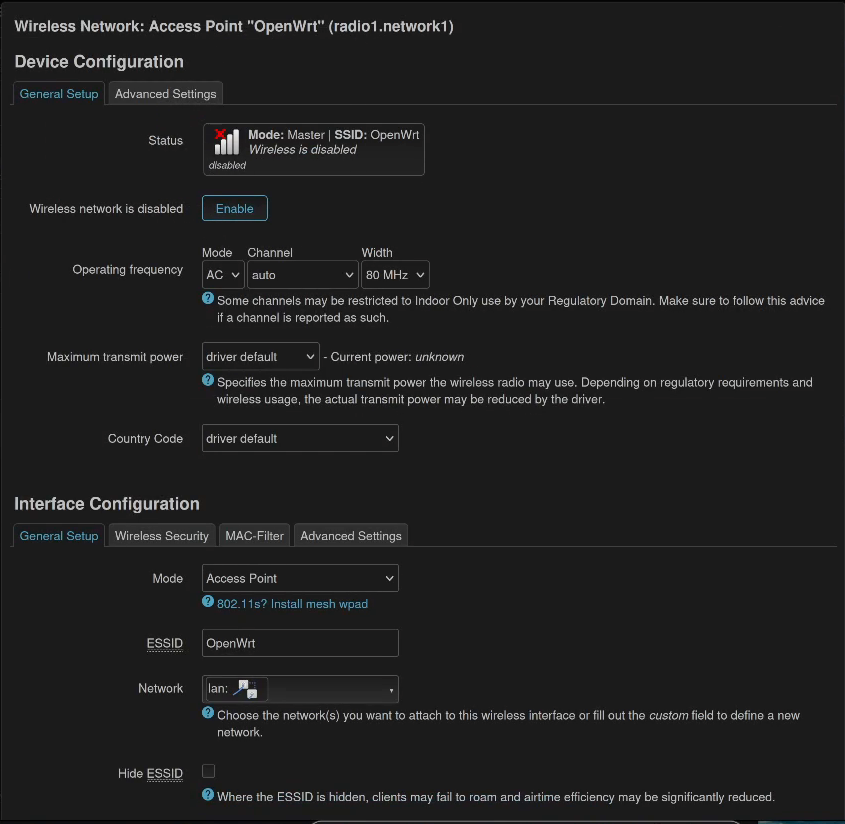
\includegraphics[width=\linewidth]{figures/N09_luci_wifi_24ghz.png}
  \caption[Cấu hình bộ phát 2,4 GHz trên LuCI]{Cấu hình bộ phát 2,4~GHz trên LuCI: mã quốc gia VN, Mode N, kênh~6,
  độ rộng 20~MHz, \ac{ssid} \texttt{25CLC04-N09}, bảo mật WPA2-PSK với mã hóa
  CCMP.}
  \label{fig:luci-wifi24}
\end{figure}

\begin{figure}[htbp]
  \centering
  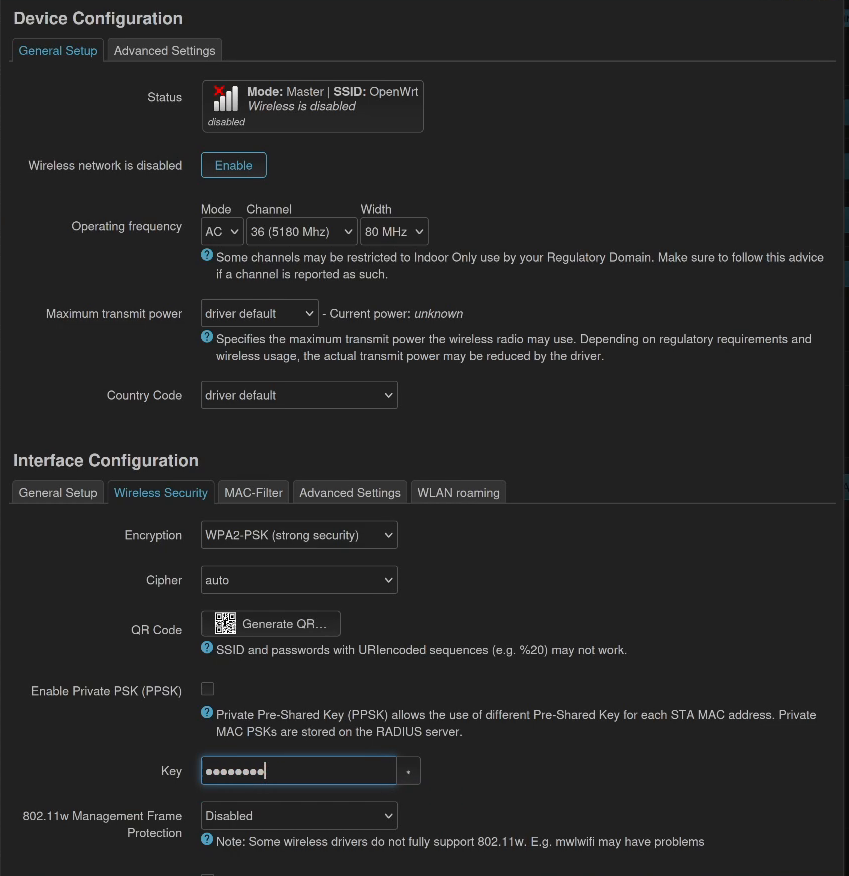
\includegraphics[width=\linewidth]{figures/N09_luci_wifi_5ghz.png}
  \caption[Cấu hình bộ phát 5 GHz trên LuCI]{Cấu hình bộ phát 5~GHz trên LuCI: chế độ AC, kênh~36, độ rộng 80~MHz,
  \ac{ssid} \texttt{25CLC04-N09-5G}.}
  \label{fig:luci-wifi5}
\end{figure}

\begin{figure}[htbp]
  \centering
  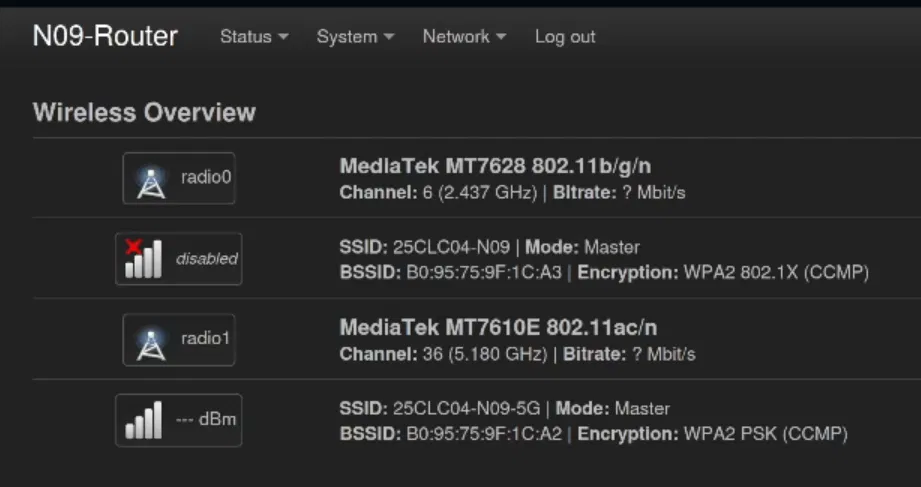
\includegraphics[width=\linewidth]{figures/N09_luci_wireless_overview.png}
  \caption[Hai bộ phát đang hoạt động trên trang Wireless]{Trang Wireless sau khi \emph{Save \& Apply}: hai bộ phát (MediaTek
  MT7628 2,4~GHz và MT7610E 5~GHz) đều đang phát, mỗi bộ phát có một
  \ac{bssid} riêng.}
  \label{fig:luci-overview}
\end{figure}

Cấu hình cấp địa chỉ được kiểm chứng bằng danh sách thuê DHCP trên router
(Hình~\ref{fig:luci-leases}) và bằng việc đặt địa chỉ IP tĩnh theo địa chỉ MAC
cho máy bàn (Hình~\ref{fig:luci-static}). Bảng~\ref{tab:dhcp-leases} tổng hợp
danh sách thiết bị đọc được từ hai nguồn này và từ sơ đồ
Hình~\ref{fig:sodo-n09}.

\begin{figure}[htbp]
  \centering
  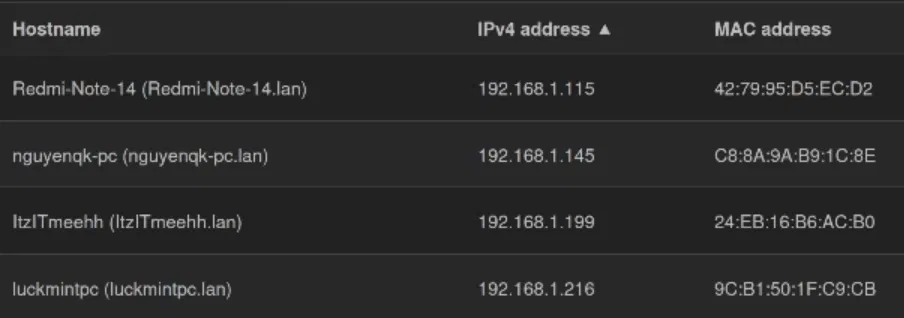
\includegraphics[width=\linewidth]{figures/N09_luci_dhcp_leases.png}
  \caption[Danh sách thuê DHCP thực tế trên N09-Router]{Danh sách thuê DHCP thực tế trên N09-Router: bốn thiết bị của nhóm đã
  nhận địa chỉ trong dải \texttt{192.168.1.0/24}.}
  \label{fig:luci-leases}
\end{figure}

\begin{figure}[htbp]
  \centering
  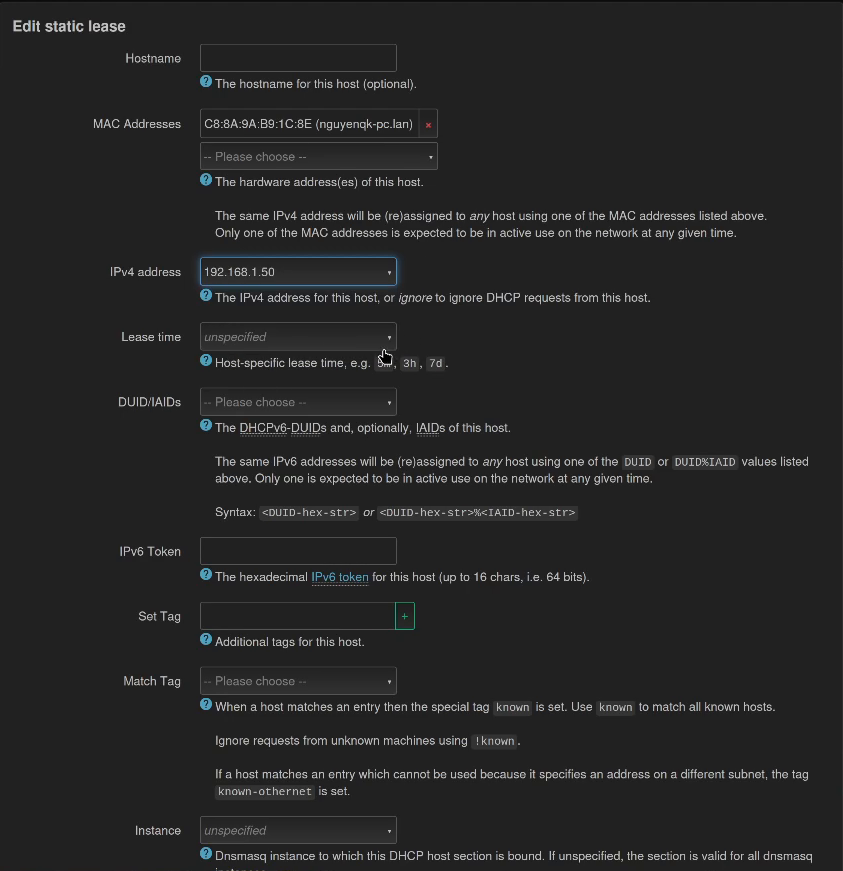
\includegraphics[width=\linewidth]{figures/N09_luci_static_lease.png}
  \caption[Đặt IP tĩnh (Static Lease) cho máy bàn]{Đặt IP tĩnh theo địa chỉ MAC (\emph{Static Lease}) cho máy bàn với địa
  chỉ \texttt{192.168.1.50}.}
  \label{fig:luci-static}
\end{figure}

\begin{table}[htbp]
  \centering\footnotesize
  \caption{Thiết bị nhận địa chỉ từ N09-Router (đọc từ \emph{Active DHCP
  Leases}).}
  \label{tab:dhcp-leases}
  \begin{tabularx}{\linewidth}{@{} L{1.0} L{0.8} L{1.15} L{1.05} @{}}
    \toprule
    \textbf{Hostname} & \textbf{Địa chỉ IPv4} & \textbf{Địa chỉ MAC} &
    \textbf{Thiết bị / kết nối} \\
    \midrule
    \texttt{luckmintpc} & \texttt{192.168.1.216} & \texttt{9C:B1:50:1F:C9:CB} &
      Máy bàn Linux Mint, nối cáp Ethernet vào cổng \ac{lan} \\
    \texttt{nguyenk-pc} & \texttt{192.168.1.145} & \texttt{C8:8A:9A:B9:1C:8E} &
      Laptop Arch Linux, Wi-Fi 5~GHz \\
    \texttt{lzITmeehh} & \texttt{192.168.1.199} & \texttt{24:EB:16:B6:AC:B0} &
      Điện thoại Android, Wi-Fi 5~GHz \\
    \texttt{Redmi-Note-14} & \texttt{192.168.1.115} & \texttt{42:79:95:D5:EC:D2} &
      Điện thoại Redmi Note 14, Wi-Fi 5~GHz \\
    \bottomrule
  \end{tabularx}
\end{table}

\subsection{Minh chứng kết nối thiết bị và kiểm tra chéo}

Sau khi cả bốn thiết bị vào mạng, máy bàn (nguồn đo) lần lượt ping tới từng thiết
bị để kiểm tra khả năng liên lạc qua router (Hình~\ref{fig:ping-shot}). Kết quả
chi tiết ở Bảng~\ref{tab:ping-crosscheck}: hai thiết bị di động phản hồi đủ 4/4
gói, còn thiết bị Android \texttt{lzITmeehh} không phản hồi trong lần đo này dù
vẫn còn trong danh sách thuê DHCP.

\begin{figure}[htbp]
  \centering
  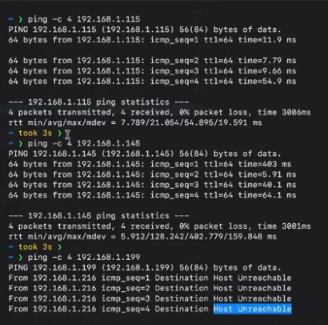
\includegraphics[width=\linewidth]{figures/N09_ping_crosscheck.png}
  \caption[Kiểm tra chéo bằng ping từ máy bàn tới các thiết bị]{Kiểm tra chéo bằng \texttt{ping} từ máy bàn tới các thiết bị trong
  mạng: hai thiết bị phản hồi đủ 4/4 gói, một thiết bị Android trả về
  \emph{Destination Host Unreachable}.}
  \label{fig:ping-shot}
\end{figure}

Ngoài ra, trên máy bàn còn kiểm tra bằng \texttt{nmcli device wifi} để xem danh
sách mạng và kênh đang dùng, và mở trình duyệt để xác nhận truy cập được trang
web khi cổng WAN đã nối. Ảnh chụp màn hình của từng điện thoại (phần cài đặt
Wi-Fi) sẽ được nhóm bổ sung; hiện minh chứng cho các thiết bị này là bảng thuê
DHCP và kết quả ping ở trên.

\subsection{Minh chứng mô hình Ad-hoc (IBSS) hai nút}
\label{subsec:evidence-adhoc}

Trước hết, khả năng hỗ trợ của hệ điều hành được kiểm tra trên máy chủ vật lý
chạy Windows~11. Lệnh \texttt{netsh wlan show drivers} trả về dòng
\emph{Hosted network supported: No} (Hình~\ref{fig:win-hosted}), xác nhận rằng
nền tảng Windows không còn hỗ trợ chế độ ngang hàng, phù hợp với nhận định trong
Mục~\ref{sec:arch}. Vì vậy mạng Ad-hoc được triển khai trên Linux theo quy trình
tại Mục~\ref{sec:adhoc-config}.

\begin{figure}[htbp]
  \centering
  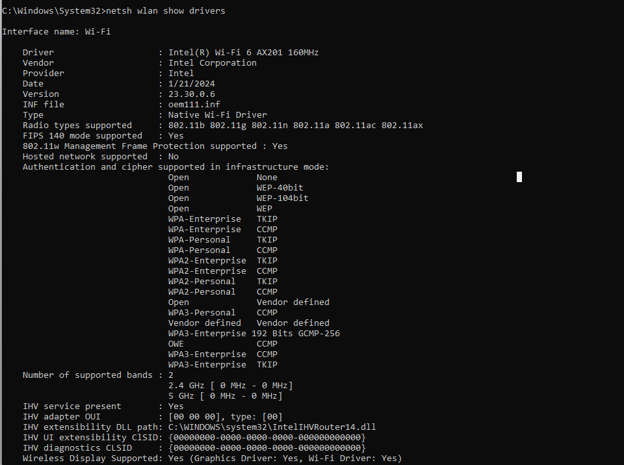
\includegraphics[width=\linewidth]{figures/Picture1.png}
  \caption[Kiểm tra hỗ trợ Ad-hoc trên Windows 11]{Kết quả \texttt{netsh wlan show drivers} trên Windows~11 với dòng
  ``Hosted network supported: No'', cho thấy hệ điều hành không hỗ trợ chế độ
  Ad-hoc.}
  \label{fig:win-hosted}
\end{figure}

Hai card mạng không dây ảo được tạo bằng module \texttt{mac80211\_hwsim} với
tham số \texttt{radios=2}. Kết quả \texttt{iw dev}
(Hình~\ref{fig:hwsim-radios}) xuất hiện hai radio độc lập \texttt{phy\#0} và
\texttt{phy\#1} cùng hai giao diện \texttt{wlan0}, \texttt{wlan1}; giao diện
\texttt{P2P-device} đi kèm \texttt{phy\#1} do trình điều khiển tự tạo để phục vụ
Wi-Fi Direct và không ảnh hưởng đến kết nối Ad-hoc.

\begin{figure}[htbp]
  \centering
  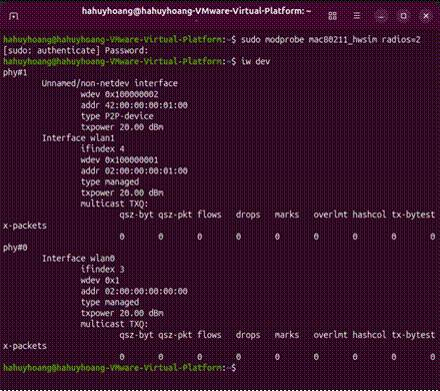
\includegraphics[width=\linewidth]{figures/Picture2.png}
  \caption[Hai radio ảo sau khi nạp \texttt{mac80211\_hwsim}]{Kết quả \texttt{iw dev} sau khi nạp module
  \texttt{mac80211\_hwsim radios=2}: hai radio ảo \texttt{phy\#0} (wlan0) và
  \texttt{phy\#1} (wlan1) được khởi tạo.}
  \label{fig:hwsim-radios}
\end{figure}

Để hai giao diện không dùng chung bảng định tuyến và chuyển gói qua loopback,
mỗi radio được tách vào một network namespace riêng (Hình~\ref{fig:netns}), nhờ
đó mỗi radio hoạt động như một máy tính độc lập.

\begin{figure}[htbp]
  \centering
  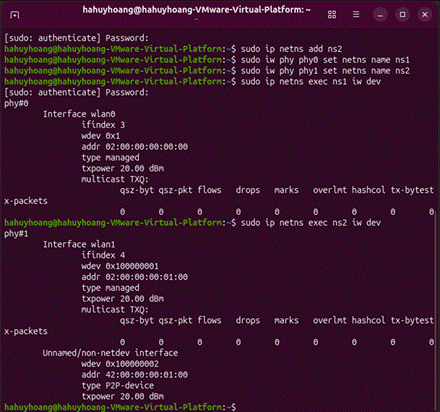
\includegraphics[width=\linewidth]{figures/Picture3.png}
  \caption[Mỗi radio trong một network namespace riêng]{Mỗi radio được gán vào một network namespace riêng: \texttt{ns1} chỉ
  thấy \texttt{phy\#0}, \texttt{ns2} chỉ thấy \texttt{phy\#1}.}
  \label{fig:netns}
\end{figure}

Hai nút được chuyển sang chế độ \ac{ibss}, cùng tham gia một mạng Ad-hoc trên tần
số 2437~MHz (kênh~6) và được gán địa chỉ \texttt{10.0.0.1/24},
\texttt{10.0.0.2/24} (Hình~\ref{fig:adhoc-config}). Lần chạy đầu tiên dùng
\ac{ssid} \texttt{demoAdhoc} như trong ảnh; bản quay minh chứng sau đó dùng
\ac{ssid} \texttt{N09-AdHoc} với cùng kênh và cùng dải địa chỉ, nên hai bộ minh
chứng nhất quán về tham số kỹ thuật.

\begin{figure}[htbp]
  \centering
  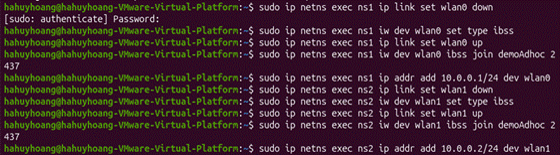
\includegraphics[width=\linewidth]{figures/Picture4.png}
  \caption[Chuỗi lệnh cấu hình chế độ IBSS]{Chuỗi lệnh cấu hình chế độ IBSS cho Node~1 (\texttt{ns1},
  \texttt{wlan0}) và Node~2 (\texttt{ns2}, \texttt{wlan1}).}
  \label{fig:adhoc-config}
\end{figure}

Kết quả kiểm tra ở Hình~\ref{fig:adhoc-check} cho thấy \texttt{wlan0} đang ở
\texttt{type IBSS}, \ac{ssid} của mạng Ad-hoc, kênh~6 (2437~MHz), độ rộng
20~MHz; lệnh \texttt{station dump} ghi nhận nút còn lại với MAC
\texttt{02:00:00:00:01:00} đã ở trạng thái \emph{authorized} và
\emph{associated}, tức hai nút đã nhận ra nhau ở tầng 802.11.

\begin{figure}[htbp]
  \centering
  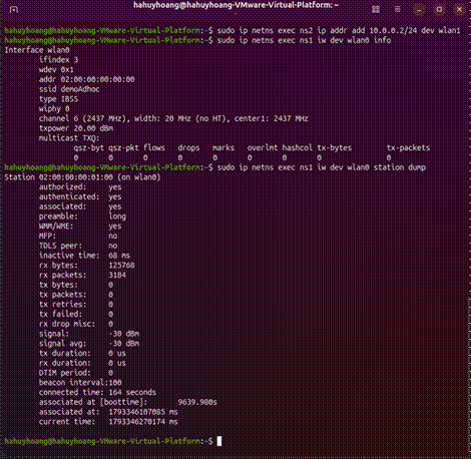
\includegraphics[width=\linewidth]{figures/Picture5.png}
  \caption[Kết quả iw info và station dump]{Kết quả \texttt{iw dev wlan0 info} (type IBSS, kênh~6) và
  \texttt{station dump} (nút lân cận \texttt{02:00:00:00:01:00} đã authenticated
  và associated).}
  \label{fig:adhoc-check}
\end{figure}

Cuối cùng, lệnh ping bốn gói giữa hai nút (Hình~\ref{fig:adhoc-ping}) nhận đủ
4/4 phản hồi, tỉ lệ mất gói 0\,\%, chứng minh mạng Ad-hoc đã hoạt động ở cả tầng
liên kết dữ liệu và tầng mạng.

\begin{figure}[htbp]
  \centering
  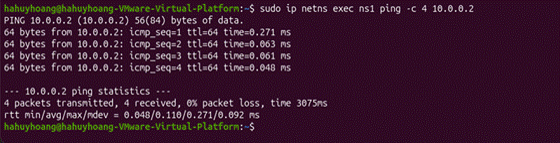
\includegraphics[width=\linewidth]{figures/Picture6.png}
  \caption[Kết quả ping giữa hai nút Ad-hoc]{Kết quả \texttt{ping -c 4 10.0.0.2} từ Node~1 sang Node~2: 4 gói gửi,
  4 gói nhận, mất gói 0\,\%.}
  \label{fig:adhoc-ping}
\end{figure}

\clearpage
\section{Kết quả thử nghiệm và thảo luận}
\label{sec:experiment}

\subsection{Mục tiêu và phạm vi thử nghiệm}
Mục tiêu của phần thử nghiệm là kiểm chứng bằng thực nghiệm hai nội dung lý
thuyết đã trình bày: (i) mô hình hạ tầng cho phép nhiều thiết bị đầu cuối cùng
truy cập tài nguyên qua một \ac{ap} trung tâm, có cấp địa chỉ tập trung và có
bảo mật hiện đại; (ii) mô hình Ad-hoc (\ac{ibss}) cho phép hai thiết bị liên lạc
trực tiếp với nhau mà không cần \ac{ap}. Phần (i) được thực hiện trên router thật
TP-Link Archer C20 v5 chạy OpenWrt với bốn thiết bị đầu cuối; phần (ii) được thực
hiện trên máy ảo Ubuntu vì các thiết bị thật của nhóm đều không còn hỗ trợ
\ac{ibss}.

\subsection{Thiết bị và mô hình thử nghiệm}
Môi trường của hai phần thử nghiệm được tóm tắt trong
Bảng~\ref{tab:moitruong-thunghiem}.

\begin{table}[htbp]
  \centering\footnotesize
  \caption{Môi trường thử nghiệm của hai mô hình.}
  \label{tab:moitruong-thunghiem}
  \begin{tabularx}{\linewidth}{@{} L{0.65} L{1.2} L{1.15} @{}}
    \toprule
    \textbf{Hạng mục} & \textbf{Mô hình hạ tầng} & \textbf{Mô hình Ad-hoc} \\
    \midrule
    Thiết bị trung tâm & TP-Link Archer C20 v5, OpenWrt, tên máy
      \texttt{N09-Router} & Không có \ac{ap} \\
    Giao diện vô tuyến & MT7628 (2,4~GHz, 802.11b/g/n) và MT7610E (5~GHz,
      802.11ac) & Hai card ảo \texttt{phy\#0}, \texttt{phy\#1} do
      \texttt{mac80211\_hwsim} sinh ra \\
    Băng tần, kênh & Kênh~6 (2,4~GHz) và kênh~36 (5~GHz) & Kênh~6 (2437~MHz),
      độ rộng 20~MHz \\
    \ac{ssid} & \texttt{25CLC04-N09} và \texttt{25CLC04-N09-5G} &
      \texttt{N09-AdHoc} \\
    Địa chỉ IP & DHCP \texttt{192.168.1.0/24}, cổng \texttt{192.168.1.1} &
      Tĩnh: \texttt{10.0.0.1/24} và \texttt{10.0.0.2/24} \\
    Bảo mật & WPA2-PSK, mã hóa CCMP (AES) & Mạng mở (không \ac{wep}, không
      WPA2/WPA3) \\
    Thiết bị tham gia & Máy bàn có dây, một laptop và hai điện thoại & Hai
      network namespace trên một máy ảo Ubuntu 22.04 \\
    \bottomrule
  \end{tabularx}
\end{table}

\subsection{Quy trình và kết quả kiểm tra}

\paragraph{Kiểm tra mô hình hạ tầng.} Quy trình gồm: cấu hình router
(Mục~\ref{sec:configuration-guide}), cấp địa chỉ cho thiết bị, kiểm tra liên lạc
với cổng mặc định và giữa các thiết bị, rồi thử các chức năng quản lý. Kết quả
cấp địa chỉ ở Bảng~\ref{tab:dhcp-leases}; kết quả kiểm tra chéo ở
Bảng~\ref{tab:ping-crosscheck}.

\begin{table}[htbp]
  \centering\footnotesize
  \caption{Kết quả ping chéo trong mạng hạ tầng (nguồn: máy bàn
  \texttt{192.168.1.216}).}
  \label{tab:ping-crosscheck}
  \begin{tabularx}{\linewidth}{@{} L{0.85} L{1.0} L{0.75} L{1.4} @{}}
    \toprule
    \textbf{Đích} & \textbf{Thiết bị} & \textbf{Gói nhận} &
    \textbf{RTT min/avg/max/mdev (ms)} \\
    \midrule
    \texttt{192.168.1.115} & Redmi Note 14, Wi-Fi 5~GHz & 4/4 (0\,\%) &
      7,789 / 21,054 / 54,895 / 19,591 \\
    \texttt{192.168.1.145} & Laptop Arch Linux, Wi-Fi 5~GHz & 4/4 (0\,\%) &
      5,912 / 128,242 / 402,779 / 159,848 \\
    \texttt{192.168.1.199} & Điện thoại Android, Wi-Fi 5~GHz & 0/4
      (100\,\%) & Không có: cả bốn gói trả về \emph{Destination Host
      Unreachable} \\
    \bottomrule
  \end{tabularx}
\end{table}

\paragraph{Kiểm tra mô hình Ad-hoc.} Kết quả kiểm tra mạng Ad-hoc hai nút được
tổng hợp ở Bảng~\ref{tab:adhoc-results}.

\begin{table}[htbp]
  \centering\footnotesize
  \caption{Kết quả kiểm tra mạng Ad-hoc hai nút.}
  \label{tab:adhoc-results}
  \begin{tabularx}{\linewidth}{@{} L{0.8} L{0.9} L{1.3} @{}}
    \toprule
    \textbf{Nội dung kiểm tra} & \textbf{Lệnh} & \textbf{Kết quả quan sát} \\
    \midrule
    Giao diện ở chế độ Ad-hoc & \texttt{iw dev wlan0 info} &
      \texttt{type IBSS}, kênh~6 (2437~MHz), độ rộng 20~MHz \\
    Phát hiện nút lân cận & \texttt{station dump} &
      MAC \texttt{02:00:00:00:01:00}, \emph{authorized} và \emph{associated} bằng
      \emph{yes}, cường độ tín hiệu $-30$~dBm, chu kỳ beacon 100~ms \\
    Liên lạc một chiều & \texttt{ping -c 4 10.0.0.2} &
      4 gói gửi, 4 gói nhận, mất gói 0\,\%, RTT cỡ 0,05--0,27~ms \\
    Liên lạc hai chiều & ping từ Node~2 về \texttt{10.0.0.1} &
      Nhận đủ phản hồi, mất gói 0\,\% \\
    \bottomrule
  \end{tabularx}
\end{table}

\subsection{Thảo luận, hạn chế và hướng khắc phục}
\begin{itemize}[leftmargin=*]
  \item \textbf{Mô hình hạ tầng hoạt động đúng lý thuyết.} Router cấp địa chỉ
    DHCP cho bốn thiết bị, hai bộ phát có \ac{bssid} riêng, và các thiết bị liên
    lạc được với nhau qua router. Các chức năng quản lý ở
    Bảng~\ref{tab:chucnang-router} đều cho kết quả quan sát đúng như mong đợi,
    gồm cả trường hợp mạng khách bị chặn truy cập trang quản trị.
  \item \textbf{Độ trễ Wi-Fi cao và dao động mạnh so với mạng có dây.} RTT tới
    hai điện thoại ở mức 21--128~ms trung bình, có gói lên tới 402~ms, trong khi
    mạng có dây thường dưới 1~ms. Nguyên nhân là cơ chế tiết kiệm điện của thiết
    bị di động và việc phải tranh chấp kênh theo \ac{csmaca}; đây cũng là lý do
    một gói đầu tiên thường chậm do phải phân giải ARP.
  \item \textbf{Một thiết bị không phản hồi dù vẫn còn trong danh sách thuê
    DHCP.} Điện thoại \texttt{lzITmeehh} trả về \emph{Destination Host
    Unreachable} cho cả bốn gói trong lần đo. Đây là bài học thực nghiệm quan
    trọng: bản ghi DHCP chỉ chứng minh thiết bị đã từng nhận địa chỉ, không
    chứng minh thiết bị đang trực tuyến; muốn kết luận phải đối chiếu thêm danh
    sách trạm liên kết (\emph{Associated Stations}) hoặc ping lại.
  \item \textbf{Mô hình Ad-hoc bị giới hạn bởi nền tảng.} Cả Windows~11, Android
    và macOS đều không còn hỗ trợ \ac{ibss}, nên thử nghiệm buộc phải chạy trên
    Linux với card ảo. Điều này khẳng định nhận định ở Mục~\ref{sec:arch} rằng
    Ad-hoc gần như đã rời khỏi thiết bị tiêu dùng.
  \item \textbf{Độ trễ trong mô hình Ad-hoc không đại diện cho Wi-Fi thật.}
    \texttt{mac80211\_hwsim} truyền khung bằng phần mềm trong nhân hệ điều hành,
    không có suy hao, khoảng cách hay di chuyển, nên RTT 0,05--0,27~ms chỉ chứng
    minh đường truyền logic hoạt động. Mô phỏng cũng không thể hiện được nhiễu
    hay chuyển vùng.
  \item \textbf{Hướng khắc phục.} Với mô hình hạ tầng: đo thêm thông lượng bằng
    \texttt{iperf3}, đo suy hao theo khoảng cách và thử chuyển vùng giữa hai
    \ac{ap}. Với mô hình Ad-hoc: lặp lại trên hai máy Linux thật có card hỗ trợ
    \ac{ibss} và thử dạng nhiều chặng (MANET) với giao thức định tuyến AODV hoặc
    OLSR.
\end{itemize}

\endgroup

\section{Kết luận}
Phần báo cáo lý thuyết trình bày các khái niệm WLAN, tiêu chuẩn IEEE 802.11,
các thành phần và mô hình triển khai, giải pháp kết nối thiết bị, nguyên tắc
cấu hình và bảo mật. Nhóm sẽ bổ sung minh chứng và kết quả kiểm tra sau khi
hoàn tất thực nghiệm; không xem nội dung mẫu là kết quả đã đo kiểm.

\clearpage
\renewcommand{\refname}{Tài liệu tham khảo}
\bibliographystyle{alpha}
\bibliography{references}

\clearpage
\section{Tỷ lệ đóng góp và minh chứng chữ ký}
Tỷ lệ cần được nhóm thống nhất theo công việc thực tế và tổng cộng bằng 100\%.
\begin{center}
\begin{tabularx}{\linewidth}{c X c c}
  \toprule
  STT & Họ và tên & Đóng góp (\%) & Chữ ký \\
  \midrule
  1 & \rule{0pt}{0.8cm} & & \\
  2 & \rule{0pt}{0.8cm} & & \\
  3 & \rule{0pt}{0.8cm} & & \\
  4 & \rule{0pt}{0.8cm} & & \\
  5 & \rule{0pt}{0.8cm} & & \\
  6 & \rule{0pt}{0.8cm} & & \\
  \midrule
  & Tổng & 100\% & \\
  \bottomrule
\end{tabularx}
\end{center}

\clearpage
\appendix
% =====================================================================
% A_abbreviations.tex -- generated automatically by the acro package
% =====================================================================
\section{Danh sách từ viết tắt}
\label{app:abbr}

\printacronyms[heading=none]

\clearpage
% B_terminology.tex -- concise English--Vietnamese WLAN terminology
% =====================================================================
\section{Thuật ngữ chuyên ngành Anh--Việt}
\label{app:terms}

\begingroup
\small
\newcolumntype{L}[1]{>{\hsize=#1\hsize\raggedright\arraybackslash}X}
\newcommand{\catrow}[1]{%
  \multicolumn{3}{@{}l@{}}{\textbf{\large #1}} \\*
  \midrule
}

\begin{xltabular}{\linewidth}{@{} L{0.8} L{0.8} L{1.4} @{}}
  \caption{Các thuật ngữ WLAN Anh--Việt thường dùng.}
  \label{tab:terms}\\
  \toprule
  \textbf{Thuật ngữ tiếng Anh (viết tắt)} & \textbf{Tiếng Việt} &
  \textbf{Giải thích ngắn}\\
  \midrule
  \endfirsthead
  \multicolumn{3}{@{}l}{\small\textsl{Bảng~\thetable\ (tiếp theo)}}\\
  \toprule
  \textbf{Thuật ngữ tiếng Anh (viết tắt)} & \textbf{Tiếng Việt} &
  \textbf{Giải thích ngắn}\\
  \midrule
  \endhead
  \midrule
  \multicolumn{3}{r@{}}{\small\textsl{tiếp tục ở trang sau}}\\
  \endfoot
  \bottomrule
  \endlastfoot

  \catrow{Mạng và kiến trúc}
  Local Area Network (LAN) & Mạng cục bộ & Mạng truyền thông phục vụ trong phạm vi địa lý giới hạn\\
  Wireless Local Area Network (WLAN) & Mạng cục bộ không dây & Mạng cục bộ sử dụng sóng vô tuyến thay cho đường dây cáp\\
  Wi-Fi & Mạng không dây Wi-Fi & Nhãn hiệu của Wi-Fi Alliance chứng nhận cho các thiết bị đạt chuẩn 802.11\\
  Access Point (AP) & Điểm truy cập & Thiết bị bắc cầu kết nối các trạm không dây vào mạng có dây\\
  Wireless station (STA) & Trạm không dây & Thiết bị được trang bị bộ thu phát vô tuyến theo chuẩn 802.11\\
  Wireless LAN Controller (WLC) & Bộ điều khiển mạng không dây & Thiết bị quản lý và kiểm soát tập trung nhiều AP dạng lightweight\\
  Basic Service Set (BSS) & Tập dịch vụ cơ bản & Một AP cùng tập hợp các trạm không dây đã thiết lập liên kết với AP đó\\
  BSS Identifier (BSSID) & Mã định danh BSS & Mã nhận diện duy nhất cho một BSS, thông thường là địa chỉ MAC của AP\\
  Extended Service Set (ESS) & Tập dịch vụ mở rộng & Hệ thống gồm nhiều BSS liên kết qua mạng phân phối và dùng chung SSID\\
  Service Set Identifier (SSID) & Tên mạng & Chuỗi tên định danh logic được mạng không dây quảng bá\\
  Association & Liên kết & Thủ tục trạm không dây gia nhập và thiết lập liên kết với một AP\\
  Distribution System (DS) & Hệ thống phân phối & Đường trục kết nối liên thông các AP trong mạng mở rộng\\
  Roaming & Chuyển vùng & Quá trình trạm di chuyển giữa các AP mà vẫn duy trì kết nối mạng liên tục\\
  Power over Ethernet (PoE) & Cấp nguồn qua Ethernet & Công nghệ cấp nguồn điện trực tiếp cho thiết bị qua sợi cáp mạng\\
  Virtual LAN (VLAN) & Mạng LAN ảo & Kỹ thuật phân đoạn logic một mạng cục bộ vật lý thành các miền quảng bá riêng\\

  \catrow{Vô tuyến và lớp vật lý}
  Wireless medium & Môi trường truyền không dây & Môi trường truyền dẫn vô tuyến dùng chung để trao đổi khung dữ liệu\\
  Frequency & Tần số & Số chu kỳ dao động toàn phần của sóng điện từ trong một giây\\
  Band & Băng tần & Dải tần số vô tuyến được phân bổ sử dụng cho một hệ thống thông tin\\
  Channel & Kênh & Phân đoạn tần số cụ thể bên trong băng tần phục vụ một liên kết mạng\\
  Channel width & Độ rộng kênh & Bề rộng dải phổ tần số mà một kênh truyền vô tuyến chiếm dụng\\
  ISM band & Băng tần công nghiệp, khoa học và y tế & Các dải tần số không cần cấp phép như 2,4~GHz và 5~GHz\\
  Regulatory domain & Miền quản lý tần số & Khu vực quốc gia áp dụng các quy chuẩn kỹ thuật riêng về tần số và công suất\\
  Antenna gain & Độ lợi anten & Khả năng tập trung năng lượng bức xạ vô tuyến theo hướng nhất định\\
  Transmit power & Công suất phát & Mức công suất sóng vô tuyến phát ra tại cổng anten, tính bằng dBm hoặc mW\\
  EIRP & Công suất bức xạ đẳng hướng tương đương & Công suất phát thực tế gồm công suất máy phát cộng độ lợi anten trừ suy hao cáp\\
  RSSI & Cường độ tín hiệu thu & Chỉ số biểu thị mức năng lượng tín hiệu vô tuyến đo được tại máy thu\\
  Signal-to-Noise Ratio (SNR) & Tỷ số tín hiệu trên nhiễu & Tỷ lệ giữa công suất tín hiệu hữu ích thu được so với công suất tạp âm nền\\
  Interference & Nhiễu & Tín hiệu vô tuyến ngoài ý muốn gây suy giảm chất lượng thu nhận tín hiệu\\
  Path loss & Suy hao đường truyền & Sự suy giảm mật độ công suất sóng điện từ khi truyền qua không gian\\
  Multipath & Đa đường & Hiện tượng tín hiệu truyền tới bên thu qua nhiều đường phản xạ khác nhau\\
  Fading & Pha-đinh & Sự biến thiên nhanh chóng của biên độ tín hiệu do các hiệu ứng truyền lan\\
  Modulation & Điều chế & Kỹ thuật biến đổi các đặc tính sóng mang để truyền tải dữ liệu số\\
  Coding rate & Tốc độ mã hóa & Tỷ số giữa số bit dữ liệu hữu ích thực tế trên tổng số bit truyền đi\\
  MCS & Sơ đồ điều chế và mã hóa & Bộ chỉ số xác định mức điều chế số kết hợp với tỷ lệ mã hóa kênh\\
  OFDM & Ghép kênh phân chia theo tần số trực giao & Phương pháp truyền dữ liệu trên nhiều sóng mang con trực giao nhau trong một kênh\\
  OFDMA & Đa truy cập phân chia theo tần số trực giao & Kỹ thuật phân chia các sóng mang con cho nhiều người dùng truyền nhận đồng thời\\
  MIMO & Đa đầu vào đa đầu ra & Kỹ thuật sử dụng đồng thời nhiều anten ở cả đầu phát và đầu thu vô tuyến\\
  Beamforming & Tạo búp sóng & Kỹ thuật xử lý tín hiệu nhằm tập trung búp sóng bức xạ về phía trạm nhận\\
  Throughput & Thông lượng & Tốc độ truyền dữ liệu hữu ích thực tế đến đích thành công trên mỗi giây\\
  Latency & Độ trễ & Khoảng thời gian truyền một gói dữ liệu từ điểm nguồn tới điểm đích\\

  \catrow{Điều khiển truy cập môi trường và chất lượng dịch vụ}
  Medium Access Control (MAC) & Điều khiển truy cập môi trường truyền & Lớp con điều phối quyền sử dụng môi trường kênh truyền vô tuyến dùng chung\\
  CSMA/CA & Đa truy cập tránh xung đột & Giao thức nghe sóng mang trước khi truyền kết hợp thời gian lùi ngẫu nhiên\\
  Carrier sense & Cảm nhận sóng mang & Kỹ thuật phát hiện trạng thái bận hay rỗi của môi trường truyền vô tuyến\\
  Backoff & Thời gian lùi & Thời gian tạm dừng ngẫu nhiên trước khi thử phát lại khung tin để tránh xung đột\\
  Contention Window (CW) & Cửa sổ tranh chấp & Phạm vi giá trị số nguyên dùng để lựa chọn ngẫu nhiên khoảng thời gian lùi\\
  Request to Send / Clear to Send (RTS/CTS) & Yêu cầu gửi / cho phép gửi & Thủ tục bắt tay trước nhằm bảo lưu môi trường truyền vô tuyến trước khi gửi dữ liệu\\
  Network Allocation Vector (NAV) & Vectơ phân bổ mạng & Bộ đếm thời gian được duy trì tại trạm nhằm cảm nhận sóng mang ảo\\
  Frame & Khung & Đơn vị dữ liệu giao thức ở lớp MAC được đóng gói và truyền trên sóng vô tuyến\\
  Beacon & Khung báo hiệu & Khung quản lý quảng bá định kỳ để thông báo sự hiện diện và tham số của BSS\\
  Authentication & Xác thực & Quá trình kiểm tra và xác nhận danh tính của trạm trước khi gia nhập mạng\\
  Acknowledgement (ACK) & Xác nhận & Khung điều khiển phản hồi xác nhận khung dữ liệu đã được thu nhận thành công\\
  Frame aggregation & Gộp khung & Cơ chế ghép nhiều khung dữ liệu nhỏ vào một lần truyền vô tuyến để tăng hiệu suất\\
  Quality of Service (QoS) & Chất lượng dịch vụ & Cơ chế phân loại và ưu tiên tài nguyên mạng cho các luồng dữ liệu quan trọng\\
  Access Category (AC) & Loại truy cập & Hạng mục phân loại lưu lượng theo thứ tự ưu tiên (thoại, video, thông thường, nền)\\
  Power save mode & Chế độ tiết kiệm năng lượng & Cơ chế cho phép vô tuyến chuyển sang chế độ ngủ để giảm mức tiêu thụ điện\\

  \catrow{Bảo mật}
  Confidentiality & Tính bí mật & Bảo đảm dữ liệu chỉ có thể đọc được bởi các bên được ủy quyền hợp pháp\\
  Integrity & Tính toàn vẹn & Bảo đảm dữ liệu không bị sửa đổi hay chèn thêm bất hợp pháp trong quá trình truyền\\
  Encryption & Mã hóa & Biến đổi bản rõ thành bản mã nhằm ngăn chặn việc đọc trộm nội dung thông tin\\
  Wired Equivalent Privacy (WEP) & Bảo mật tương đương mạng có dây & Chuẩn bảo mật không dây ban đầu dựa trên RC4, hiện đã lỗi thời và không an toàn\\
  Wi-Fi Protected Access (WPA) & Truy cập Wi-Fi được bảo vệ & Bộ tiêu chuẩn và chứng nhận bảo mật không dây thay thế cho WEP\\
  Advanced Encryption Standard (AES) & Chuẩn mã hóa nâng cao & Thuật toán mã hóa khối đối xứng được áp dụng bắt buộc trong WPA2 và WPA3\\
  Pre-Shared Key (PSK) & Khóa chia sẻ trước & Phương thức xác thực dùng chung mật khẩu bí mật cấu hình sẵn trên các thiết bị\\
  Simultaneous Authentication of Equals (SAE) & Xác thực đồng đẳng & Giao thức trao đổi khóa dựa trên mật khẩu có tính bảo mật chuyển tiếp trong WPA3\\
  Protected Management Frames (PMF) & Khung quản lý được bảo vệ & Cơ chế mã hóa và bảo vệ tính toàn vẹn cho các khung quản lý unicast và broadcast\\
  Pairwise Master Key (PMK) & Khóa chủ theo cặp & Khóa bí mật gốc làm cơ sở để dẫn xuất các khóa phiên tạm thời\\
  Pairwise Transient Key (PTK) & Khóa tạm thời theo cặp & Tập hợp các khóa phiên đơn hướng dùng để mã hóa và kiểm tra toàn vẹn dữ liệu\\
  Extensible Authentication Protocol (EAP) & Giao thức xác thực mở rộng & Khung giao thức hỗ trợ đóng gói nhiều phương thức xác thực người dùng khác nhau\\
  RADIUS & Dịch vụ xác thực người dùng từ xa & Giao thức AAA tiêu chuẩn dùng kết hợp với 802.1X để xác thực người dùng tập trung\\
  Virtual Private Network (VPN) & Mạng riêng ảo & Đường hầm mã hóa bảo mật truyền tải lưu lượng qua môi trường mạng không tin cậy\\
  Rogue AP & AP trái phép & Điểm truy cập trái phép được gắn vào mạng nội bộ mà không có sự phê duyệt\\
  Evil twin & AP song sinh độc hại & Điểm truy cập mạo danh phát cùng SSID của mạng hợp pháp nhằm đánh cắp thông tin\\
  Wireless Intrusion Prevention System (WIPS) & Hệ thống ngăn chặn xâm nhập không dây & Hệ thống giám sát phổ tần vô tuyến để phát hiện và ngăn chặn các cuộc tấn công\\

  \catrow{Triển khai và vận hành}
  Site survey & Khảo sát hiện trường & Hoạt động đo đạc thực địa và mô phỏng vùng phủ sóng trước khi triển khai mạng\\
  Heat map & Bản đồ nhiệt & Bản đồ biểu diễn trực quan cường độ tín hiệu hoặc thông lượng trên mặt bằng khu vực\\
  Coverage hole & Vùng lõm sóng & Khu vực có cường độ tín hiệu vô tuyến yếu dưới ngưỡng yêu cầu hoạt động\\
  Capacity & Dung lượng & Khả năng xử lý tổng lưu lượng và đáp ứng số lượng kết nối đồng thời của hệ thống\\
  Cell overlap & Độ chồng lấn ô & Phần không gian phủ sóng giao thoa giữa các AP lân cận để hỗ trợ chuyển vùng êm dịu\\
  Channel plan & Quy hoạch kênh & Kế hoạch phân bổ tần số kênh truyền cho các AP nhằm triệt tiêu nhiễu đồng kênh\\
  Airtime & Thời gian chiếm kênh & Khoảng thời gian mà một trạm hoặc AP chiếm dụng môi trường truyền vô tuyến\\
  Channel utilization & Mức sử dụng kênh & Tỷ lệ phần trăm thời gian mà kênh vô tuyến ở trạng thái bận do truyền nhận tín hiệu\\
  Retry rate & Tỷ lệ truyền lại & Tỷ lệ phần trăm các khung dữ liệu phải gửi lại do xảy ra lỗi hoặc xung đột\\
  Packet capture & Bắt gói tin & Kỹ thuật thu thập và ghi lại toàn bộ khung dữ liệu vô tuyến để chẩn đoán lỗi\\
  Monitor mode & Chế độ giám sát & Chế độ hoạt động cho phép card mạng thu nhận mọi khung dữ liệu trên kênh mà không cần liên kết\\
  Firmware & Phần mềm điều khiển & Phần mềm nhúng chuyên dụng điều khiển hoạt động phần cứng của thiết bị mạng\\
\end{xltabular}
\endgroup


\end{document}
